% Options for packages loaded elsewhere
\PassOptionsToPackage{unicode}{hyperref}
\PassOptionsToPackage{hyphens}{url}
\PassOptionsToPackage{dvipsnames,svgnames,x11names}{xcolor}
%
\documentclass[
  letterpaper,
  DIV=11,
  numbers=noendperiod,
  oneside]{scrreprt}

\usepackage{amsmath,amssymb}
\usepackage{iftex}
\ifPDFTeX
  \usepackage[T1]{fontenc}
  \usepackage[utf8]{inputenc}
  \usepackage{textcomp} % provide euro and other symbols
\else % if luatex or xetex
  \usepackage{unicode-math}
  \defaultfontfeatures{Scale=MatchLowercase}
  \defaultfontfeatures[\rmfamily]{Ligatures=TeX,Scale=1}
\fi
\usepackage{lmodern}
\ifPDFTeX\else  
    % xetex/luatex font selection
\fi
% Use upquote if available, for straight quotes in verbatim environments
\IfFileExists{upquote.sty}{\usepackage{upquote}}{}
\IfFileExists{microtype.sty}{% use microtype if available
  \usepackage[]{microtype}
  \UseMicrotypeSet[protrusion]{basicmath} % disable protrusion for tt fonts
}{}
\makeatletter
\@ifundefined{KOMAClassName}{% if non-KOMA class
  \IfFileExists{parskip.sty}{%
    \usepackage{parskip}
  }{% else
    \setlength{\parindent}{0pt}
    \setlength{\parskip}{6pt plus 2pt minus 1pt}}
}{% if KOMA class
  \KOMAoptions{parskip=half}}
\makeatother
\usepackage{xcolor}
\usepackage[left=1in,marginparwidth=2.0666666666667in,textwidth=4.1333333333333in,marginparsep=0.3in]{geometry}
\setlength{\emergencystretch}{3em} % prevent overfull lines
\setcounter{secnumdepth}{5}
% Make \paragraph and \subparagraph free-standing
\ifx\paragraph\undefined\else
  \let\oldparagraph\paragraph
  \renewcommand{\paragraph}[1]{\oldparagraph{#1}\mbox{}}
\fi
\ifx\subparagraph\undefined\else
  \let\oldsubparagraph\subparagraph
  \renewcommand{\subparagraph}[1]{\oldsubparagraph{#1}\mbox{}}
\fi

\usepackage{color}
\usepackage{fancyvrb}
\newcommand{\VerbBar}{|}
\newcommand{\VERB}{\Verb[commandchars=\\\{\}]}
\DefineVerbatimEnvironment{Highlighting}{Verbatim}{commandchars=\\\{\}}
% Add ',fontsize=\small' for more characters per line
\usepackage{framed}
\definecolor{shadecolor}{RGB}{241,243,245}
\newenvironment{Shaded}{\begin{snugshade}}{\end{snugshade}}
\newcommand{\AlertTok}[1]{\textcolor[rgb]{0.68,0.00,0.00}{#1}}
\newcommand{\AnnotationTok}[1]{\textcolor[rgb]{0.37,0.37,0.37}{#1}}
\newcommand{\AttributeTok}[1]{\textcolor[rgb]{0.40,0.45,0.13}{#1}}
\newcommand{\BaseNTok}[1]{\textcolor[rgb]{0.68,0.00,0.00}{#1}}
\newcommand{\BuiltInTok}[1]{\textcolor[rgb]{0.00,0.23,0.31}{#1}}
\newcommand{\CharTok}[1]{\textcolor[rgb]{0.13,0.47,0.30}{#1}}
\newcommand{\CommentTok}[1]{\textcolor[rgb]{0.37,0.37,0.37}{#1}}
\newcommand{\CommentVarTok}[1]{\textcolor[rgb]{0.37,0.37,0.37}{\textit{#1}}}
\newcommand{\ConstantTok}[1]{\textcolor[rgb]{0.56,0.35,0.01}{#1}}
\newcommand{\ControlFlowTok}[1]{\textcolor[rgb]{0.00,0.23,0.31}{#1}}
\newcommand{\DataTypeTok}[1]{\textcolor[rgb]{0.68,0.00,0.00}{#1}}
\newcommand{\DecValTok}[1]{\textcolor[rgb]{0.68,0.00,0.00}{#1}}
\newcommand{\DocumentationTok}[1]{\textcolor[rgb]{0.37,0.37,0.37}{\textit{#1}}}
\newcommand{\ErrorTok}[1]{\textcolor[rgb]{0.68,0.00,0.00}{#1}}
\newcommand{\ExtensionTok}[1]{\textcolor[rgb]{0.00,0.23,0.31}{#1}}
\newcommand{\FloatTok}[1]{\textcolor[rgb]{0.68,0.00,0.00}{#1}}
\newcommand{\FunctionTok}[1]{\textcolor[rgb]{0.28,0.35,0.67}{#1}}
\newcommand{\ImportTok}[1]{\textcolor[rgb]{0.00,0.46,0.62}{#1}}
\newcommand{\InformationTok}[1]{\textcolor[rgb]{0.37,0.37,0.37}{#1}}
\newcommand{\KeywordTok}[1]{\textcolor[rgb]{0.00,0.23,0.31}{#1}}
\newcommand{\NormalTok}[1]{\textcolor[rgb]{0.00,0.23,0.31}{#1}}
\newcommand{\OperatorTok}[1]{\textcolor[rgb]{0.37,0.37,0.37}{#1}}
\newcommand{\OtherTok}[1]{\textcolor[rgb]{0.00,0.23,0.31}{#1}}
\newcommand{\PreprocessorTok}[1]{\textcolor[rgb]{0.68,0.00,0.00}{#1}}
\newcommand{\RegionMarkerTok}[1]{\textcolor[rgb]{0.00,0.23,0.31}{#1}}
\newcommand{\SpecialCharTok}[1]{\textcolor[rgb]{0.37,0.37,0.37}{#1}}
\newcommand{\SpecialStringTok}[1]{\textcolor[rgb]{0.13,0.47,0.30}{#1}}
\newcommand{\StringTok}[1]{\textcolor[rgb]{0.13,0.47,0.30}{#1}}
\newcommand{\VariableTok}[1]{\textcolor[rgb]{0.07,0.07,0.07}{#1}}
\newcommand{\VerbatimStringTok}[1]{\textcolor[rgb]{0.13,0.47,0.30}{#1}}
\newcommand{\WarningTok}[1]{\textcolor[rgb]{0.37,0.37,0.37}{\textit{#1}}}

\providecommand{\tightlist}{%
  \setlength{\itemsep}{0pt}\setlength{\parskip}{0pt}}\usepackage{longtable,booktabs,array}
\usepackage{calc} % for calculating minipage widths
% Correct order of tables after \paragraph or \subparagraph
\usepackage{etoolbox}
\makeatletter
\patchcmd\longtable{\par}{\if@noskipsec\mbox{}\fi\par}{}{}
\makeatother
% Allow footnotes in longtable head/foot
\IfFileExists{footnotehyper.sty}{\usepackage{footnotehyper}}{\usepackage{footnote}}
\makesavenoteenv{longtable}
\usepackage{graphicx}
\makeatletter
\def\maxwidth{\ifdim\Gin@nat@width>\linewidth\linewidth\else\Gin@nat@width\fi}
\def\maxheight{\ifdim\Gin@nat@height>\textheight\textheight\else\Gin@nat@height\fi}
\makeatother
% Scale images if necessary, so that they will not overflow the page
% margins by default, and it is still possible to overwrite the defaults
% using explicit options in \includegraphics[width, height, ...]{}
\setkeys{Gin}{width=\maxwidth,height=\maxheight,keepaspectratio}
% Set default figure placement to htbp
\makeatletter
\def\fps@figure{htbp}
\makeatother
\newlength{\cslhangindent}
\setlength{\cslhangindent}{1.5em}
\newlength{\csllabelwidth}
\setlength{\csllabelwidth}{3em}
\newlength{\cslentryspacingunit} % times entry-spacing
\setlength{\cslentryspacingunit}{\parskip}
\newenvironment{CSLReferences}[2] % #1 hanging-ident, #2 entry spacing
 {% don't indent paragraphs
  \setlength{\parindent}{0pt}
  % turn on hanging indent if param 1 is 1
  \ifodd #1
  \let\oldpar\par
  \def\par{\hangindent=\cslhangindent\oldpar}
  \fi
  % set entry spacing
  \setlength{\parskip}{#2\cslentryspacingunit}
 }%
 {}
\usepackage{calc}
\newcommand{\CSLBlock}[1]{#1\hfill\break}
\newcommand{\CSLLeftMargin}[1]{\parbox[t]{\csllabelwidth}{#1}}
\newcommand{\CSLRightInline}[1]{\parbox[t]{\linewidth - \csllabelwidth}{#1}\break}
\newcommand{\CSLIndent}[1]{\hspace{\cslhangindent}#1}

\KOMAoption{captions}{tableheading}
\makeatletter
\makeatother
\makeatletter
\@ifpackageloaded{bookmark}{}{\usepackage{bookmark}}
\makeatother
\makeatletter
\@ifpackageloaded{caption}{}{\usepackage{caption}}
\AtBeginDocument{%
\ifdefined\contentsname
  \renewcommand*\contentsname{Table of contents}
\else
  \newcommand\contentsname{Table of contents}
\fi
\ifdefined\listfigurename
  \renewcommand*\listfigurename{List of Figures}
\else
  \newcommand\listfigurename{List of Figures}
\fi
\ifdefined\listtablename
  \renewcommand*\listtablename{List of Tables}
\else
  \newcommand\listtablename{List of Tables}
\fi
\ifdefined\figurename
  \renewcommand*\figurename{Figure}
\else
  \newcommand\figurename{Figure}
\fi
\ifdefined\tablename
  \renewcommand*\tablename{Table}
\else
  \newcommand\tablename{Table}
\fi
}
\@ifpackageloaded{float}{}{\usepackage{float}}
\floatstyle{ruled}
\@ifundefined{c@chapter}{\newfloat{codelisting}{h}{lop}}{\newfloat{codelisting}{h}{lop}[chapter]}
\floatname{codelisting}{Listing}
\newcommand*\listoflistings{\listof{codelisting}{List of Listings}}
\makeatother
\makeatletter
\@ifpackageloaded{caption}{}{\usepackage{caption}}
\@ifpackageloaded{subcaption}{}{\usepackage{subcaption}}
\makeatother
\makeatletter
\@ifpackageloaded{tcolorbox}{}{\usepackage[skins,breakable]{tcolorbox}}
\makeatother
\makeatletter
\@ifundefined{shadecolor}{\definecolor{shadecolor}{rgb}{.97, .97, .97}}
\makeatother
\makeatletter
\makeatother
\makeatletter
\@ifpackageloaded{sidenotes}{}{\usepackage{sidenotes}}
\@ifpackageloaded{marginnote}{}{\usepackage{marginnote}}
\makeatother
\makeatletter
\makeatother
\ifLuaTeX
  \usepackage{selnolig}  % disable illegal ligatures
\fi
\IfFileExists{bookmark.sty}{\usepackage{bookmark}}{\usepackage{hyperref}}
\IfFileExists{xurl.sty}{\usepackage{xurl}}{} % add URL line breaks if available
\urlstyle{same} % disable monospaced font for URLs
\hypersetup{
  pdftitle={NCCS Research Guide},
  pdfauthor={Jesse Lecy; Hannah Martin},
  colorlinks=true,
  linkcolor={blue},
  filecolor={Maroon},
  citecolor={Blue},
  urlcolor={Blue},
  pdfcreator={LaTeX via pandoc}}

\title{NCCS Research Guide}
\author{Jesse Lecy \and Hannah Martin}
\date{2023-09-24}

\begin{document}
\maketitle
\ifdefined\Shaded\renewenvironment{Shaded}{\begin{tcolorbox}[enhanced, borderline west={3pt}{0pt}{shadecolor}, interior hidden, boxrule=0pt, sharp corners, breakable, frame hidden]}{\end{tcolorbox}}\fi

\renewcommand*\contentsname{Table of contents}
{
\hypersetup{linkcolor=}
\setcounter{tocdepth}{2}
\tableofcontents
}
\bookmarksetup{startatroot}

\hypertarget{preface}{%
\chapter*{Preface}\label{preface}}
\addcontentsline{toc}{chapter}{Preface}

\markboth{Preface}{Preface}

This is a Quarto book.

To learn more about Quarto books visit
\url{https://quarto.org/docs/books}.

\begin{Shaded}
\begin{Highlighting}[]
\DecValTok{1} \SpecialCharTok{+} \DecValTok{1}
\end{Highlighting}
\end{Shaded}

\begin{verbatim}
[1] 2
\end{verbatim}

\bookmarksetup{startatroot}

\hypertarget{introduction}{%
\chapter{Introduction}\label{introduction}}

This is a book created from markdown and executable code.

See Knuth (1984) for additional discussion of literate programming.

\begin{Shaded}
\begin{Highlighting}[]
\DecValTok{1} \SpecialCharTok{+} \DecValTok{1}
\end{Highlighting}
\end{Shaded}

\begin{verbatim}
[1] 2
\end{verbatim}

\bookmarksetup{startatroot}

\hypertarget{summary}{%
\chapter{Summary}\label{summary}}

In summary, this book has no content whatsoever.

\begin{Shaded}
\begin{Highlighting}[]
\DecValTok{1} \SpecialCharTok{+} \DecValTok{1}
\end{Highlighting}
\end{Shaded}

\begin{verbatim}
[1] 2
\end{verbatim}

\begin{Shaded}
\begin{Highlighting}[]
\NormalTok{dat}\SpecialCharTok{$}\NormalTok{hour12 }\OtherTok{\textless{}{-}} \FunctionTok{format}\NormalTok{( date.vec, }\AttributeTok{format=}\StringTok{"\%l \%p"}\NormalTok{ )}
\FunctionTok{table}\NormalTok{( dat}\SpecialCharTok{$}\NormalTok{hour12 ) }\SpecialCharTok{\%\textgreater{}\%} \FunctionTok{head}\NormalTok{() }\SpecialCharTok{\%\textgreater{}\%} \FunctionTok{pander}\NormalTok{()}

\CommentTok{\# set the levels so they are in the correct order}
\NormalTok{time.levels }\OtherTok{\textless{}{-}}
  \FunctionTok{c}\NormalTok{( }\StringTok{"12 AM"}\NormalTok{, }\StringTok{" 1 AM"}\NormalTok{, }\StringTok{" 2 AM"}\NormalTok{, }\StringTok{" 3 AM"}\NormalTok{, }\StringTok{" 4 AM"}\NormalTok{, }\StringTok{" 5 AM"}\NormalTok{, }
     \StringTok{" 6 AM"}\NormalTok{, }\StringTok{" 7 AM"}\NormalTok{, }\StringTok{" 8 AM"}\NormalTok{, }\StringTok{" 9 AM"}\NormalTok{, }\StringTok{"10 AM"}\NormalTok{, }\StringTok{"11 AM"}\NormalTok{, }
     \StringTok{"12 PM"}\NormalTok{, }\StringTok{" 1 PM"}\NormalTok{, }\StringTok{" 2 PM"}\NormalTok{, }\StringTok{" 3 PM"}\NormalTok{, }\StringTok{" 4 PM"}\NormalTok{, }\StringTok{" 5 PM"}\NormalTok{, }
     \StringTok{" 6 PM"}\NormalTok{, }\StringTok{" 7 PM"}\NormalTok{, }\StringTok{" 8 PM"}\NormalTok{, }\StringTok{" 9 PM"}\NormalTok{, }\StringTok{"10 PM"}\NormalTok{, }\StringTok{"11 PM"}\NormalTok{ )}

\NormalTok{dat}\SpecialCharTok{$}\NormalTok{hour12 }\OtherTok{\textless{}{-}} \FunctionTok{factor}\NormalTok{( dat}\SpecialCharTok{$}\NormalTok{hour12, }\AttributeTok{levels=}\NormalTok{time.levels )}
\FunctionTok{table}\NormalTok{( dat}\SpecialCharTok{$}\NormalTok{hour12 ) }\SpecialCharTok{\%\textgreater{}\%} \FunctionTok{head}\NormalTok{() }\SpecialCharTok{\%\textgreater{}\%} \FunctionTok{pander}\NormalTok{()}
\end{Highlighting}
\end{Shaded}

\begin{Shaded}
\begin{Highlighting}[]
\FunctionTok{qplot}\NormalTok{( }\AttributeTok{data=}\NormalTok{d3, }\AttributeTok{x=}\FunctionTok{as.numeric}\NormalTok{(}\FunctionTok{as.character}\NormalTok{(hour)), }\AttributeTok{y=}\NormalTok{harm ) }\SpecialCharTok{+} 
  \FunctionTok{geom\_line}\NormalTok{( }\AttributeTok{color=}\StringTok{"steelblue"}\NormalTok{, }\AttributeTok{size=}\FloatTok{0.8}\NormalTok{ ) }\SpecialCharTok{+} 
  \FunctionTok{geom\_point}\NormalTok{( }\AttributeTok{color=}\StringTok{"darkblue"}\NormalTok{, }\AttributeTok{size=}\DecValTok{3}\NormalTok{ ) }\SpecialCharTok{+} 
  \FunctionTok{geom\_hline}\NormalTok{( }\AttributeTok{yintercept=}\NormalTok{mean.harm, }\AttributeTok{color=}\StringTok{"black"}\NormalTok{ ) }\SpecialCharTok{+} 
  \FunctionTok{facet\_wrap}\NormalTok{( }\SpecialCharTok{\textasciitilde{}}\NormalTok{ age, }\AttributeTok{ncol=}\DecValTok{4}\NormalTok{ ) }\SpecialCharTok{+} 
  \FunctionTok{xlab}\NormalTok{(}\StringTok{"Time of Day (24hrs)"}\NormalTok{) }\SpecialCharTok{+} \FunctionTok{ylab}\NormalTok{(}\StringTok{"Rate of Harm"}\NormalTok{) }\SpecialCharTok{+}
  \FunctionTok{ggtitle}\NormalTok{(}\StringTok{"Proportion of Accidents Resulting in Harm"}\NormalTok{) }\SpecialCharTok{+}
  \CommentTok{\# theme\_fivethirtyeight() }
  \FunctionTok{theme\_wsj}\NormalTok{( }\AttributeTok{base\_size=}\DecValTok{10}\NormalTok{, }\AttributeTok{color=}\StringTok{"gray"}\NormalTok{ )}
\end{Highlighting}
\end{Shaded}

\bookmarksetup{startatroot}

\hypertarget{summary-1}{%
\chapter{Summary}\label{summary-1}}

In summary, this book has no content whatsoever.

\begin{Shaded}
\begin{Highlighting}[]
\DecValTok{1} \SpecialCharTok{+} \DecValTok{1}
\end{Highlighting}
\end{Shaded}

\begin{verbatim}
[1] 2
\end{verbatim}

\hypertarget{section-1}{%
\section{Section 1}\label{section-1}}

Lorem ipsum dolor sit amet, consectetur adipiscing elit, sed do eiusmod
tempor incididunt ut labore et dolore magna aliqua. Tellus rutrum tellus
pellentesque eu tincidunt tortor aliquam nulla facilisi. Sollicitudin
aliquam ultrices sagittis orci a scelerisque purus semper eget. Risus
viverra adipiscing at in tellus integer feugiat scelerisque varius. Id
consectetur purus ut faucibus pulvinar elementum. Aenean et tortor at
risus viverra adipiscing at. Ornare massa eget egestas purus viverra.
Ultrices sagittis orci a scelerisque purus semper eget duis at. Neque
egestas congue quisque egestas diam in arcu cursus. Magna ac placerat
vestibulum lectus mauris ultrices eros. Nunc lobortis mattis aliquam
faucibus purus. Lobortis elementum nibh tellus molestie. Sed libero enim
sed faucibus turpis. Id consectetur purus ut faucibus pulvinar
elementum. Id consectetur purus ut faucibus pulvinar elementum. Ut
aliquam purus sit amet. Tincidunt ornare massa eget egestas purus
viverra accumsan. Pharetra et ultrices neque ornare aenean euismod. Nec
dui nunc mattis enim ut tellus elementum. Tincidunt arcu non sodales
neque sodales ut etiam sit amet.

Aenean et tortor at risus viverra adipiscing at. Id volutpat lacus
laoreet non curabitur gravida. Diam maecenas sed enim ut sem viverra
aliquet eget. Malesuada pellentesque elit eget gravida cum sociis
natoque penatibus et. Tortor vitae purus faucibus ornare suspendisse
sed. Auctor elit sed vulputate mi sit amet mauris commodo. Orci sagittis
eu volutpat odio facilisis. Est ullamcorper eget nulla facilisi etiam
dignissim diam quis. Faucibus in ornare quam viverra orci sagittis eu.
Non nisi est sit amet facilisis magna etiam tempor. Nulla posuere
sollicitudin aliquam ultrices sagittis orci a. In tellus integer feugiat
scelerisque. Rutrum tellus pellentesque eu tincidunt tortor aliquam
nulla facilisi. Velit ut tortor pretium viverra suspendisse potenti
nullam. Lectus urna duis convallis convallis. Senectus et netus et
malesuada fames ac turpis egestas. Sed enim ut sem viverra aliquet eget
sit. Sapien nec sagittis aliquam malesuada. Nulla malesuada pellentesque
elit eget gravida.

\hypertarget{subection-1-1}{%
\subsection{Subection 1-1}\label{subection-1-1}}

Volutpat ac tincidunt vitae semper quis lectus nulla at. Nulla facilisi
cras fermentum odio eu feugiat pretium nibh. Ornare quam viverra orci
sagittis eu volutpat odio. Cum sociis natoque penatibus et magnis dis
parturient montes. Erat imperdiet sed euismod nisi porta lorem mollis
aliquam. Eu non diam phasellus vestibulum lorem sed risus ultricies
tristique. Scelerisque in dictum non consectetur a erat nam at lectus.
Sodales neque sodales ut etiam sit amet nisl. Faucibus turpis in eu mi.
Egestas dui id ornare arcu odio. Interdum consectetur libero id faucibus
nisl tincidunt eget. Eu ultrices vitae auctor eu. Ut etiam sit amet
nisl. Risus viverra adipiscing at in tellus integer feugiat scelerisque
varius.

Suspendisse sed nisi lacus sed viverra tellus in. Pretium quam vulputate
dignissim suspendisse in est ante in. Augue eget arcu dictum varius duis
at. Sed arcu non odio euismod. Volutpat diam ut venenatis tellus in.
Turpis nunc eget lorem dolor sed viverra ipsum nunc. Purus viverra
accumsan in nisl nisi scelerisque eu. Vel quam elementum pulvinar etiam
non. Auctor augue mauris augue neque. Sed arcu non odio euismod. Natoque
penatibus et magnis dis. In ante metus dictum at. Risus viverra
adipiscing at in tellus.

\hypertarget{subsection-1-2}{%
\subsection{Subsection 1-2}\label{subsection-1-2}}

Enim neque volutpat ac tincidunt. Curabitur vitae nunc sed velit
dignissim sodales ut eu. Elit at imperdiet dui accumsan sit. Velit
laoreet id donec ultrices tincidunt arcu non sodales neque. Proin nibh
nisl condimentum id venenatis a condimentum. Lacinia at quis risus sed
vulputate odio ut enim blandit. Cursus in hac habitasse platea dictumst
quisque sagittis purus sit. Vitae semper quis lectus nulla at volutpat.
Vel pharetra vel turpis nunc eget lorem. Nascetur ridiculus mus mauris
vitae ultricies leo integer. Consequat mauris nunc congue nisi vitae
suscipit tellus. Egestas purus viverra accumsan in nisl nisi
scelerisque. Aliquam vestibulum morbi blandit cursus risus at. Viverra
vitae congue eu consequat ac felis donec. Lacus suspendisse faucibus
interdum posuere.

\begin{Shaded}
\begin{Highlighting}[]
\FunctionTok{library}\NormalTok{(ggridges)}
\end{Highlighting}
\end{Shaded}

\begin{verbatim}
Warning: package 'ggridges' was built under R version 4.1.3
\end{verbatim}

\begin{Shaded}
\begin{Highlighting}[]
\FunctionTok{library}\NormalTok{(ggplot2)}
\end{Highlighting}
\end{Shaded}

\begin{verbatim}
Warning: package 'ggplot2' was built under R version 4.1.3
\end{verbatim}

\begin{Shaded}
\begin{Highlighting}[]
\CommentTok{\# Diamonds dataset is provided by R natively}
\CommentTok{\#head(diamonds)}
 
\CommentTok{\# basic example}
\FunctionTok{ggplot}\NormalTok{(diamonds, }\FunctionTok{aes}\NormalTok{(}\AttributeTok{x =}\NormalTok{ price, }\AttributeTok{y =}\NormalTok{ cut, }\AttributeTok{fill =}\NormalTok{ cut)) }\SpecialCharTok{+}
  \FunctionTok{geom\_density\_ridges}\NormalTok{() }\SpecialCharTok{+}
  \FunctionTok{theme\_ridges}\NormalTok{() }\SpecialCharTok{+} 
  \FunctionTok{theme}\NormalTok{(}\AttributeTok{legend.position =} \StringTok{"none"}\NormalTok{)}
\end{Highlighting}
\end{Shaded}

\begin{verbatim}
Picking joint bandwidth of 458
\end{verbatim}

\begin{figure}[H]

{\centering 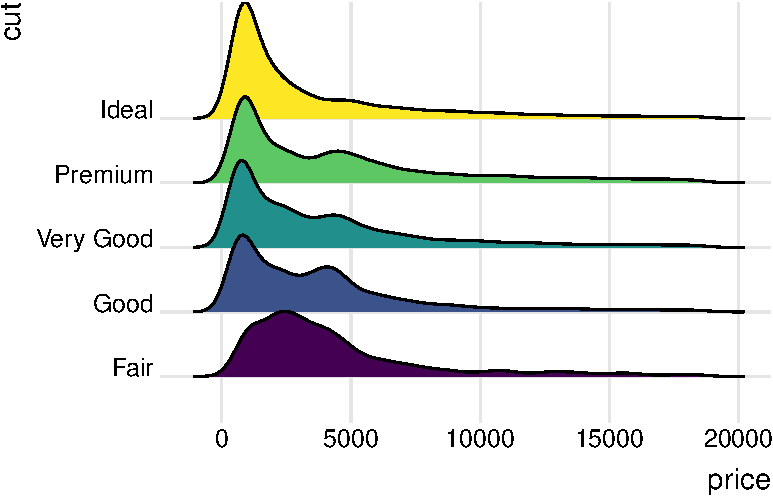
\includegraphics{standard-01_files/figure-pdf/unnamed-chunk-2-1.pdf}

}

\end{figure}

\hypertarget{section-2}{%
\section{Section 2}\label{section-2}}

Lorem ipsum dolor sit amet, consectetur adipiscing elit, sed do eiusmod
tempor incididunt ut labore et dolore magna aliqua. Nisl rhoncus mattis
rhoncus urna neque viverra justo nec ultrices. Fermentum iaculis eu non
diam phasellus. In hendrerit gravida rutrum quisque non tellus orci ac
auctor. Purus semper eget duis at. Ornare quam viverra orci sagittis.
Congue eu consequat ac felis donec et odio pellentesque diam. Ac
tincidunt vitae semper quis lectus nulla at volutpat diam. Placerat orci
nulla pellentesque dignissim enim sit amet venenatis urna. Egestas sed
tempus urna et pharetra pharetra massa massa. Massa tincidunt nunc
pulvinar sapien et ligula. Duis ultricies lacus sed turpis tincidunt id
aliquet. At augue eget arcu dictum varius duis. Tristique risus nec
feugiat in fermentum posuere urna nec tincidunt. Velit scelerisque in
dictum non consectetur a erat nam at. Est ullamcorper eget nulla
facilisi etiam dignissim diam. Enim lobortis scelerisque fermentum dui
faucibus in. Senectus et netus et malesuada fames ac turpis. Adipiscing
tristique risus nec feugiat.

\begin{Shaded}
\begin{Highlighting}[]
\FunctionTok{qplot}\NormalTok{( }\AttributeTok{data=}\NormalTok{d3, }\AttributeTok{x=}\FunctionTok{as.numeric}\NormalTok{(}\FunctionTok{as.character}\NormalTok{(hour)), }\AttributeTok{y=}\NormalTok{harm ) }\SpecialCharTok{+} 
  \FunctionTok{geom\_line}\NormalTok{( }\AttributeTok{color=}\StringTok{"steelblue"}\NormalTok{, }\AttributeTok{size=}\FloatTok{0.8}\NormalTok{ ) }\SpecialCharTok{+} 
  \FunctionTok{geom\_point}\NormalTok{( }\AttributeTok{color=}\StringTok{"darkblue"}\NormalTok{, }\AttributeTok{size=}\DecValTok{3}\NormalTok{ ) }\SpecialCharTok{+} 
  \FunctionTok{geom\_hline}\NormalTok{( }\AttributeTok{yintercept=}\NormalTok{mean.harm, }\AttributeTok{color=}\StringTok{"black"}\NormalTok{ ) }\SpecialCharTok{+} 
  \FunctionTok{facet\_wrap}\NormalTok{( }\SpecialCharTok{\textasciitilde{}}\NormalTok{ age, }\AttributeTok{ncol=}\DecValTok{4}\NormalTok{ ) }\SpecialCharTok{+} 
  \FunctionTok{xlab}\NormalTok{(}\StringTok{"Time of Day (24hrs)"}\NormalTok{) }\SpecialCharTok{+} \FunctionTok{ylab}\NormalTok{(}\StringTok{"Rate of Harm"}\NormalTok{) }\SpecialCharTok{+}
  \FunctionTok{ggtitle}\NormalTok{(}\StringTok{"Proportion of Accidents Resulting in Harm"}\NormalTok{) }\SpecialCharTok{+}
  \CommentTok{\# theme\_fivethirtyeight() }
  \FunctionTok{theme\_wsj}\NormalTok{( }\AttributeTok{base\_size=}\DecValTok{10}\NormalTok{, }\AttributeTok{color=}\StringTok{"gray"}\NormalTok{ )}
\end{Highlighting}
\end{Shaded}

Lorem donec massa sapien faucibus et molestie ac feugiat sed. Fermentum
odio eu feugiat pretium nibh ipsum. Neque sodales ut etiam sit amet nisl
purus. Arcu cursus euismod quis viverra nibh cras pulvinar mattis nunc.
Aliquam eleifend mi in nulla posuere sollicitudin aliquam ultrices.
Iaculis urna id volutpat lacus laoreet. Adipiscing diam donec adipiscing
tristique risus nec. Scelerisque felis imperdiet proin fermentum leo vel
orci porta non. Ultricies tristique nulla aliquet enim tortor at auctor
urna. Lacus luctus accumsan tortor posuere ac ut. Sagittis vitae et leo
duis ut. Sed lectus vestibulum mattis ullamcorper velit. A cras semper
auctor neque vitae. Sed tempus urna et pharetra. Vulputate dignissim
suspendisse in est ante in.

\begin{marginfigure}

{\centering 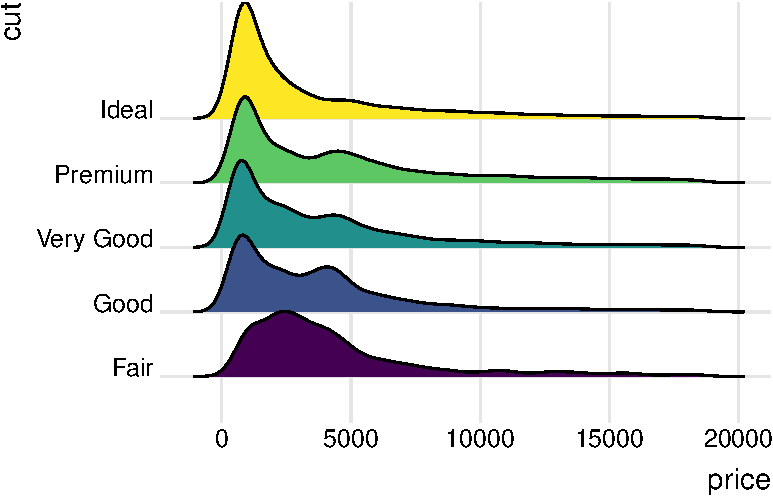
\includegraphics{standard-01_files/figure-pdf/unnamed-chunk-4-1.pdf}

}

\caption{An informative figure capture here.}

\end{marginfigure}

Vestibulum lectus mauris ultrices eros in cursus turpis massa. Commodo
odio aenean sed adipiscing diam. Tellus at urna condimentum mattis
pellentesque id nibh. Scelerisque purus semper eget duis at tellus.
Pellentesque id nibh tortor id. Nunc faucibus a pellentesque sit. Amet
tellus cras adipiscing enim eu. Nunc non blandit massa enim nec dui nunc
mattis enim. Dolor sit amet consectetur adipiscing. Tristique senectus
et netus et malesuada fames ac turpis egestas. Lobortis elementum nibh
tellus molestie.

\hypertarget{citation-style}{%
\section{Citation Style}\label{citation-style}}

See the
\href{https://quarto.org/docs/authoring/footnotes-and-citations.html\#sec-citations}{citation
style guide}:

\begin{longtable}[]{@{}
  >{\raggedright\arraybackslash}p{(\columnwidth - 4\tabcolsep) * \real{0.3750}}
  >{\raggedright\arraybackslash}p{(\columnwidth - 4\tabcolsep) * \real{0.3472}}
  >{\raggedright\arraybackslash}p{(\columnwidth - 4\tabcolsep) * \real{0.2778}}@{}}
\toprule\noalign{}
\begin{minipage}[b]{\linewidth}\raggedright
Markdown Format
\end{minipage} & \begin{minipage}[b]{\linewidth}\raggedright
Output (default Chicago Style)
\end{minipage} & \begin{minipage}[b]{\linewidth}\raggedright
Output (custom csi)
\end{minipage} \\
\midrule\noalign{}
\endhead
\bottomrule\noalign{}
\endlastfoot
Blah Blah (see \textbf{knuth1984?}; also \textbf{wickham2015?}) & Blah
Blah (see Knuth 1984, 33--35; also Wickham 2015, chap.~1) & Blah Blah
see {[}1{]}, pp.~33-35; also {[}1{]}, chap.~1 \\
Blah Blah (\textbf{knuth1984?} and passim) & Blah Blah (Knuth 1984,
33--35, 38--39 and passim) & Blah Blah {[}1{]}, pp.~33-35, 38-39 and
passim \\
Blah Blah (\textbf{wickham2015?}; \textbf{knuth1984?}). & Blah Blah
(Wickham 2015; Knuth 1984). & Blah Blah {[}1, 2{]}. \\
Wickham says blah (\textbf{wickham2015?}) & Wickham says blah (2015) &
Wickham says blah {[}1{]} \\
(\textbf{knuth1984?}) says blah. & Knuth (1984) says blah. & {[}1{]}
says blah. \\
(\textbf{knuth1984?}) says blah. & Knuth (1984, 33) says blah. & {[}1{]}
{[}p.~33{]} says blah. \\
\end{longtable}

\bookmarksetup{startatroot}

\hypertarget{summary-2}{%
\chapter{Summary}\label{summary-2}}

In summary, this book has no content whatsoever.

\begin{Shaded}
\begin{Highlighting}[]
\DecValTok{1} \SpecialCharTok{+} \DecValTok{1}
\end{Highlighting}
\end{Shaded}

\begin{verbatim}
[1] 2
\end{verbatim}

\begin{Shaded}
\begin{Highlighting}[]
\NormalTok{dat}\SpecialCharTok{$}\NormalTok{hour12 }\OtherTok{\textless{}{-}} \FunctionTok{format}\NormalTok{( date.vec, }\AttributeTok{format=}\StringTok{"\%l \%p"}\NormalTok{ )}
\FunctionTok{table}\NormalTok{( dat}\SpecialCharTok{$}\NormalTok{hour12 ) }\SpecialCharTok{\%\textgreater{}\%} \FunctionTok{head}\NormalTok{() }\SpecialCharTok{\%\textgreater{}\%} \FunctionTok{pander}\NormalTok{()}

\CommentTok{\# set the levels so they are in the correct order}
\NormalTok{time.levels }\OtherTok{\textless{}{-}}
  \FunctionTok{c}\NormalTok{( }\StringTok{"12 AM"}\NormalTok{, }\StringTok{" 1 AM"}\NormalTok{, }\StringTok{" 2 AM"}\NormalTok{, }\StringTok{" 3 AM"}\NormalTok{, }\StringTok{" 4 AM"}\NormalTok{, }\StringTok{" 5 AM"}\NormalTok{, }
     \StringTok{" 6 AM"}\NormalTok{, }\StringTok{" 7 AM"}\NormalTok{, }\StringTok{" 8 AM"}\NormalTok{, }\StringTok{" 9 AM"}\NormalTok{, }\StringTok{"10 AM"}\NormalTok{, }\StringTok{"11 AM"}\NormalTok{, }
     \StringTok{"12 PM"}\NormalTok{, }\StringTok{" 1 PM"}\NormalTok{, }\StringTok{" 2 PM"}\NormalTok{, }\StringTok{" 3 PM"}\NormalTok{, }\StringTok{" 4 PM"}\NormalTok{, }\StringTok{" 5 PM"}\NormalTok{, }
     \StringTok{" 6 PM"}\NormalTok{, }\StringTok{" 7 PM"}\NormalTok{, }\StringTok{" 8 PM"}\NormalTok{, }\StringTok{" 9 PM"}\NormalTok{, }\StringTok{"10 PM"}\NormalTok{, }\StringTok{"11 PM"}\NormalTok{ )}

\NormalTok{dat}\SpecialCharTok{$}\NormalTok{hour12 }\OtherTok{\textless{}{-}} \FunctionTok{factor}\NormalTok{( dat}\SpecialCharTok{$}\NormalTok{hour12, }\AttributeTok{levels=}\NormalTok{time.levels )}
\FunctionTok{table}\NormalTok{( dat}\SpecialCharTok{$}\NormalTok{hour12 ) }\SpecialCharTok{\%\textgreater{}\%} \FunctionTok{head}\NormalTok{() }\SpecialCharTok{\%\textgreater{}\%} \FunctionTok{pander}\NormalTok{()}
\end{Highlighting}
\end{Shaded}

\begin{Shaded}
\begin{Highlighting}[]
\FunctionTok{qplot}\NormalTok{( }\AttributeTok{data=}\NormalTok{d3, }\AttributeTok{x=}\FunctionTok{as.numeric}\NormalTok{(}\FunctionTok{as.character}\NormalTok{(hour)), }\AttributeTok{y=}\NormalTok{harm ) }\SpecialCharTok{+} 
  \FunctionTok{geom\_line}\NormalTok{( }\AttributeTok{color=}\StringTok{"steelblue"}\NormalTok{, }\AttributeTok{size=}\FloatTok{0.8}\NormalTok{ ) }\SpecialCharTok{+} 
  \FunctionTok{geom\_point}\NormalTok{( }\AttributeTok{color=}\StringTok{"darkblue"}\NormalTok{, }\AttributeTok{size=}\DecValTok{3}\NormalTok{ ) }\SpecialCharTok{+} 
  \FunctionTok{geom\_hline}\NormalTok{( }\AttributeTok{yintercept=}\NormalTok{mean.harm, }\AttributeTok{color=}\StringTok{"black"}\NormalTok{ ) }\SpecialCharTok{+} 
  \FunctionTok{facet\_wrap}\NormalTok{( }\SpecialCharTok{\textasciitilde{}}\NormalTok{ age, }\AttributeTok{ncol=}\DecValTok{4}\NormalTok{ ) }\SpecialCharTok{+} 
  \FunctionTok{xlab}\NormalTok{(}\StringTok{"Time of Day (24hrs)"}\NormalTok{) }\SpecialCharTok{+} \FunctionTok{ylab}\NormalTok{(}\StringTok{"Rate of Harm"}\NormalTok{) }\SpecialCharTok{+}
  \FunctionTok{ggtitle}\NormalTok{(}\StringTok{"Proportion of Accidents Resulting in Harm"}\NormalTok{) }\SpecialCharTok{+}
  \CommentTok{\# theme\_fivethirtyeight() }
  \FunctionTok{theme\_wsj}\NormalTok{( }\AttributeTok{base\_size=}\DecValTok{10}\NormalTok{, }\AttributeTok{color=}\StringTok{"gray"}\NormalTok{ )}
\end{Highlighting}
\end{Shaded}

\bookmarksetup{startatroot}

\hypertarget{summary-3}{%
\chapter{Summary}\label{summary-3}}

In summary, this book has no content whatsoever.

\begin{Shaded}
\begin{Highlighting}[]
\DecValTok{1} \SpecialCharTok{+} \DecValTok{1}
\end{Highlighting}
\end{Shaded}

\begin{verbatim}
[1] 2
\end{verbatim}

\begin{Shaded}
\begin{Highlighting}[]
\NormalTok{dat}\SpecialCharTok{$}\NormalTok{hour12 }\OtherTok{\textless{}{-}} \FunctionTok{format}\NormalTok{( date.vec, }\AttributeTok{format=}\StringTok{"\%l \%p"}\NormalTok{ )}
\FunctionTok{table}\NormalTok{( dat}\SpecialCharTok{$}\NormalTok{hour12 ) }\SpecialCharTok{\%\textgreater{}\%} \FunctionTok{head}\NormalTok{() }\SpecialCharTok{\%\textgreater{}\%} \FunctionTok{pander}\NormalTok{()}

\CommentTok{\# set the levels so they are in the correct order}
\NormalTok{time.levels }\OtherTok{\textless{}{-}}
  \FunctionTok{c}\NormalTok{( }\StringTok{"12 AM"}\NormalTok{, }\StringTok{" 1 AM"}\NormalTok{, }\StringTok{" 2 AM"}\NormalTok{, }\StringTok{" 3 AM"}\NormalTok{, }\StringTok{" 4 AM"}\NormalTok{, }\StringTok{" 5 AM"}\NormalTok{, }
     \StringTok{" 6 AM"}\NormalTok{, }\StringTok{" 7 AM"}\NormalTok{, }\StringTok{" 8 AM"}\NormalTok{, }\StringTok{" 9 AM"}\NormalTok{, }\StringTok{"10 AM"}\NormalTok{, }\StringTok{"11 AM"}\NormalTok{, }
     \StringTok{"12 PM"}\NormalTok{, }\StringTok{" 1 PM"}\NormalTok{, }\StringTok{" 2 PM"}\NormalTok{, }\StringTok{" 3 PM"}\NormalTok{, }\StringTok{" 4 PM"}\NormalTok{, }\StringTok{" 5 PM"}\NormalTok{, }
     \StringTok{" 6 PM"}\NormalTok{, }\StringTok{" 7 PM"}\NormalTok{, }\StringTok{" 8 PM"}\NormalTok{, }\StringTok{" 9 PM"}\NormalTok{, }\StringTok{"10 PM"}\NormalTok{, }\StringTok{"11 PM"}\NormalTok{ )}

\NormalTok{dat}\SpecialCharTok{$}\NormalTok{hour12 }\OtherTok{\textless{}{-}} \FunctionTok{factor}\NormalTok{( dat}\SpecialCharTok{$}\NormalTok{hour12, }\AttributeTok{levels=}\NormalTok{time.levels )}
\FunctionTok{table}\NormalTok{( dat}\SpecialCharTok{$}\NormalTok{hour12 ) }\SpecialCharTok{\%\textgreater{}\%} \FunctionTok{head}\NormalTok{() }\SpecialCharTok{\%\textgreater{}\%} \FunctionTok{pander}\NormalTok{()}
\end{Highlighting}
\end{Shaded}

\begin{Shaded}
\begin{Highlighting}[]
\FunctionTok{qplot}\NormalTok{( }\AttributeTok{data=}\NormalTok{d3, }\AttributeTok{x=}\FunctionTok{as.numeric}\NormalTok{(}\FunctionTok{as.character}\NormalTok{(hour)), }\AttributeTok{y=}\NormalTok{harm ) }\SpecialCharTok{+} 
  \FunctionTok{geom\_line}\NormalTok{( }\AttributeTok{color=}\StringTok{"steelblue"}\NormalTok{, }\AttributeTok{size=}\FloatTok{0.8}\NormalTok{ ) }\SpecialCharTok{+} 
  \FunctionTok{geom\_point}\NormalTok{( }\AttributeTok{color=}\StringTok{"darkblue"}\NormalTok{, }\AttributeTok{size=}\DecValTok{3}\NormalTok{ ) }\SpecialCharTok{+} 
  \FunctionTok{geom\_hline}\NormalTok{( }\AttributeTok{yintercept=}\NormalTok{mean.harm, }\AttributeTok{color=}\StringTok{"black"}\NormalTok{ ) }\SpecialCharTok{+} 
  \FunctionTok{facet\_wrap}\NormalTok{( }\SpecialCharTok{\textasciitilde{}}\NormalTok{ age, }\AttributeTok{ncol=}\DecValTok{4}\NormalTok{ ) }\SpecialCharTok{+} 
  \FunctionTok{xlab}\NormalTok{(}\StringTok{"Time of Day (24hrs)"}\NormalTok{) }\SpecialCharTok{+} \FunctionTok{ylab}\NormalTok{(}\StringTok{"Rate of Harm"}\NormalTok{) }\SpecialCharTok{+}
  \FunctionTok{ggtitle}\NormalTok{(}\StringTok{"Proportion of Accidents Resulting in Harm"}\NormalTok{) }\SpecialCharTok{+}
  \CommentTok{\# theme\_fivethirtyeight() }
  \FunctionTok{theme\_wsj}\NormalTok{( }\AttributeTok{base\_size=}\DecValTok{10}\NormalTok{, }\AttributeTok{color=}\StringTok{"gray"}\NormalTok{ )}
\end{Highlighting}
\end{Shaded}

\bookmarksetup{startatroot}

\hypertarget{summary-4}{%
\chapter{Summary}\label{summary-4}}

In summary, this book has no content whatsoever.

\begin{Shaded}
\begin{Highlighting}[]
\DecValTok{1} \SpecialCharTok{+} \DecValTok{1}
\end{Highlighting}
\end{Shaded}

\begin{verbatim}
[1] 2
\end{verbatim}

\begin{Shaded}
\begin{Highlighting}[]
\NormalTok{dat}\SpecialCharTok{$}\NormalTok{hour12 }\OtherTok{\textless{}{-}} \FunctionTok{format}\NormalTok{( date.vec, }\AttributeTok{format=}\StringTok{"\%l \%p"}\NormalTok{ )}
\FunctionTok{table}\NormalTok{( dat}\SpecialCharTok{$}\NormalTok{hour12 ) }\SpecialCharTok{\%\textgreater{}\%} \FunctionTok{head}\NormalTok{() }\SpecialCharTok{\%\textgreater{}\%} \FunctionTok{pander}\NormalTok{()}

\CommentTok{\# set the levels so they are in the correct order}
\NormalTok{time.levels }\OtherTok{\textless{}{-}}
  \FunctionTok{c}\NormalTok{( }\StringTok{"12 AM"}\NormalTok{, }\StringTok{" 1 AM"}\NormalTok{, }\StringTok{" 2 AM"}\NormalTok{, }\StringTok{" 3 AM"}\NormalTok{, }\StringTok{" 4 AM"}\NormalTok{, }\StringTok{" 5 AM"}\NormalTok{, }
     \StringTok{" 6 AM"}\NormalTok{, }\StringTok{" 7 AM"}\NormalTok{, }\StringTok{" 8 AM"}\NormalTok{, }\StringTok{" 9 AM"}\NormalTok{, }\StringTok{"10 AM"}\NormalTok{, }\StringTok{"11 AM"}\NormalTok{, }
     \StringTok{"12 PM"}\NormalTok{, }\StringTok{" 1 PM"}\NormalTok{, }\StringTok{" 2 PM"}\NormalTok{, }\StringTok{" 3 PM"}\NormalTok{, }\StringTok{" 4 PM"}\NormalTok{, }\StringTok{" 5 PM"}\NormalTok{, }
     \StringTok{" 6 PM"}\NormalTok{, }\StringTok{" 7 PM"}\NormalTok{, }\StringTok{" 8 PM"}\NormalTok{, }\StringTok{" 9 PM"}\NormalTok{, }\StringTok{"10 PM"}\NormalTok{, }\StringTok{"11 PM"}\NormalTok{ )}

\NormalTok{dat}\SpecialCharTok{$}\NormalTok{hour12 }\OtherTok{\textless{}{-}} \FunctionTok{factor}\NormalTok{( dat}\SpecialCharTok{$}\NormalTok{hour12, }\AttributeTok{levels=}\NormalTok{time.levels )}
\FunctionTok{table}\NormalTok{( dat}\SpecialCharTok{$}\NormalTok{hour12 ) }\SpecialCharTok{\%\textgreater{}\%} \FunctionTok{head}\NormalTok{() }\SpecialCharTok{\%\textgreater{}\%} \FunctionTok{pander}\NormalTok{()}
\end{Highlighting}
\end{Shaded}

\begin{Shaded}
\begin{Highlighting}[]
\FunctionTok{qplot}\NormalTok{( }\AttributeTok{data=}\NormalTok{d3, }\AttributeTok{x=}\FunctionTok{as.numeric}\NormalTok{(}\FunctionTok{as.character}\NormalTok{(hour)), }\AttributeTok{y=}\NormalTok{harm ) }\SpecialCharTok{+} 
  \FunctionTok{geom\_line}\NormalTok{( }\AttributeTok{color=}\StringTok{"steelblue"}\NormalTok{, }\AttributeTok{size=}\FloatTok{0.8}\NormalTok{ ) }\SpecialCharTok{+} 
  \FunctionTok{geom\_point}\NormalTok{( }\AttributeTok{color=}\StringTok{"darkblue"}\NormalTok{, }\AttributeTok{size=}\DecValTok{3}\NormalTok{ ) }\SpecialCharTok{+} 
  \FunctionTok{geom\_hline}\NormalTok{( }\AttributeTok{yintercept=}\NormalTok{mean.harm, }\AttributeTok{color=}\StringTok{"black"}\NormalTok{ ) }\SpecialCharTok{+} 
  \FunctionTok{facet\_wrap}\NormalTok{( }\SpecialCharTok{\textasciitilde{}}\NormalTok{ age, }\AttributeTok{ncol=}\DecValTok{4}\NormalTok{ ) }\SpecialCharTok{+} 
  \FunctionTok{xlab}\NormalTok{(}\StringTok{"Time of Day (24hrs)"}\NormalTok{) }\SpecialCharTok{+} \FunctionTok{ylab}\NormalTok{(}\StringTok{"Rate of Harm"}\NormalTok{) }\SpecialCharTok{+}
  \FunctionTok{ggtitle}\NormalTok{(}\StringTok{"Proportion of Accidents Resulting in Harm"}\NormalTok{) }\SpecialCharTok{+}
  \CommentTok{\# theme\_fivethirtyeight() }
  \FunctionTok{theme\_wsj}\NormalTok{( }\AttributeTok{base\_size=}\DecValTok{10}\NormalTok{, }\AttributeTok{color=}\StringTok{"gray"}\NormalTok{ )}
\end{Highlighting}
\end{Shaded}

\bookmarksetup{startatroot}

\hypertarget{foundations-trusts-and-grant-making-organizations}{%
\chapter{Foundations, Trusts, and Grant-Making
Organizations}\label{foundations-trusts-and-grant-making-organizations}}

This chapter explains NCCS's taxonomy for foundations, trusts, and
grant-making organizations:

\begin{longtable}[]{@{}
  >{\raggedright\arraybackslash}p{(\columnwidth - 12\tabcolsep) * \real{0.0052}}
  >{\raggedright\arraybackslash}p{(\columnwidth - 12\tabcolsep) * \real{0.0135}}
  >{\raggedright\arraybackslash}p{(\columnwidth - 12\tabcolsep) * \real{0.0232}}
  >{\raggedright\arraybackslash}p{(\columnwidth - 12\tabcolsep) * \real{0.0285}}
  >{\raggedright\arraybackslash}p{(\columnwidth - 12\tabcolsep) * \real{0.0120}}
  >{\raggedright\arraybackslash}p{(\columnwidth - 12\tabcolsep) * \real{0.0936}}
  >{\raggedright\arraybackslash}p{(\columnwidth - 12\tabcolsep) * \real{0.8240}}@{}}
\toprule\noalign{}
\begin{minipage}[b]{\linewidth}\raggedright
Value
\end{minipage} & \begin{minipage}[b]{\linewidth}\raggedright
Group
\end{minipage} & \begin{minipage}[b]{\linewidth}\raggedright
Subtype
\end{minipage} & \begin{minipage}[b]{\linewidth}\raggedright
501(c)(3) private foundation subtype
\end{minipage} & \begin{minipage}[b]{\linewidth}\raggedright
Subsection
\end{minipage} & \begin{minipage}[b]{\linewidth}\raggedright
Description
\end{minipage} & \begin{minipage}[b]{\linewidth}\raggedright
Formula
\end{minipage} \\
\midrule\noalign{}
\endhead
\bottomrule\noalign{}
\endlastfoot
0 & not a foundation & NA & NA & NA & Not a foundation, trust, or
grant-making organization & FNDNCD != 2 \& FNDNCD != 3 \& FNDNCD != 4 \&
NTEECC != ``T20'' \& NTEECC != ``T21'' \& NTEECC != ``T22'' \& NTEECC !=
``T23'' \& NTEECC != ``T30'' \& NTEECC != ``T31'' \& NTEECC != ``A11''
\& NTEECC != ``B11'' \& NTEECC != ``C11'' \& NTEECC != ``D11'' \& NTEECC
!= ``E11'' \& NTEECC != ``F11'' \& NTEECC != ``G11'' \& NTEECC !=
``H11'' \& NTEECC != ``I11'' \& NTEECC != ``J11'' \& NTEECC != ``K11''
\& NTEECC != ``L11'' \& NTEECC != ``M11'' \& NTEECC != ``N11'' \& NTEECC
!= ``O11'' \& NTEECC != ``P11'' \& NTEECC != ``Q11'' \& NTEECC !=
``R11'' \& NTEECC != ``S11'' \& NTEECC != ``T11'' \& NTEECC != ``U11''
\& NTEECC != ``V11'' \& NTEECC != ``W11'' \& NTEECC != ``X11'' \& NTEECC
!= ``Y11'' \& NTEECC != ``A12'' \& NTEECC != ``B12'' \& NTEECC !=
``C12'' \& NTEECC != ``D12'' \& NTEECC != ``E12'' \& NTEECC != ``F12''
\& NTEECC != ``G12'' \& NTEECC != ``H12'' \& NTEECC != ``I12'' \& NTEECC
!= ``J12'' \& NTEECC != ``K12'' \& NTEECC != ``L12'' \& NTEECC !=
``M12'' \& NTEECC != ``N12'' \& NTEECC != ``O12'' \& NTEECC != ``P12''
\& NTEECC != ``Q12'' \& NTEECC != ``R12'' \& NTEECC != ``S12'' \& NTEECC
!= ``T12'' \& NTEECC != ``U12'' \& NTEECC != ``V12'' \& NTEECC !=
``W12'' \& NTEECC != ``X12'' \& NTEECC != ``Y12'' \& SUBSECCD != 90 \&
SUBSECCD != 91 \& SUBSECCD != 92 \\
1 & private & corporate & private operating & 501(c)(3) & 501(c)(3)
private: private operating foundation (IRS status) \& corporate
foundation (NTEE code) & SUBSECCD == 3 \& FNDNCD == 3 \& NTEECC ==
``T21'' \\
2 & private & corporate & exempt operating & 501(c)(3) & 501(c)(3)
private: exempt operating foundation (IRS status) \& corporate
foundation (NTEE code) & SUBSECCD == 3 \& FNDNCD == 2 \& NTEECC ==
``T21'' \\
3 & private & corporate & grant-making (private nonoperating) &
501(c)(3) & 501(c)(3) private: grant-making (private nonoperating)
foundation (IRS status) \& corporate foundation (NTEE code) & SUBSECCD
== 3 \& FNDNCD == 4 \& NTEECC == ``T21'' \\
4 & private & independent & private operating & 501(c)(3) & 501(c)(3)
private: private operating foundation (IRS status) \& private
independent foundation (NTEE code) & SUBSECCD == 3 \& FNDNCD == 3 \&
NTEECC == ``T22'' \\
5 & private & independent & exempt operating & 501(c)(3) & 501(c)(3)
private: exempt operating foundation (IRS status) \& private independent
foundation (NTEE code) & SUBSECCD == 3 \& FNDNCD == 2 \& NTEECC ==
``T22'' \\
6 & private & independent & grant-making (private nonoperating) &
501(c)(3) & 501(c)(3) private: grant-making (private nonoperating)
foundation (IRS status) \& private independent foundation (NTEE code) &
SUBSECCD == 3 \& FNDNCD == 4 \& NTEECC == ``T22'' \\
7 & private & operating & private operating & 501(c)(3) & 501(c)(3)
private: private operating foundation (IRS status) \& private operating
foundation (NTEE code) & SUBSECCD == 3 \& FNDNCD == 3 \& NTEECC ==
``T23'' \\
8 & private & operating & exempt operating & 501(c)(3) & 501(c)(3)
private: exempt operating foundation (IRS status) \& private operating
foundation (NTEE code) & SUBSECCD == 3 \& FNDNCD == 2 \& NTEECC ==
``T23'' \\
9 & private & operating & grant-making (private nonoperating) &
501(c)(3) & 501(c)(3) private: grant-making (private nonoperating)
foundation (IRS status) \& private operating foundation (NTEE code) &
SUBSECCD == 3 \& FNDNCD == 4 \& NTEECC == ``T23'' \\
10 & private & other & private operating & 501(c)(3) & 501(c)(3)
private: private operating foundation (IRS status), other (NTEE code) &
SUBSECCD == 3 \& FNDNCD == 3 \& NTEECC != ``T21'' \& NTEECC != ``T22''
\& NTEECC != ``T23'' \\
11 & private & other & exempt operating & 501(c)(3) & 501(c)(3) private:
exempt operating foundation (IRS status), other (NTEE code) & SUBSECCD
== 3 \& FNDNCD == 2 \& NTEECC != ``T21'' \& NTEECC != ``T22'' \& NTEECC
!= ``T23'' \\
12 & private & other & grant-making (private nonoperating) & 501(c)(3) &
501(c)(3) private: grant-making (private nonoperating) foundation (IRS
status), other (NTEE code) & SUBSECCD == 3 \& FNDNCD == 4 \& NTEECC !=
``T21'' \& NTEECC != ``T22'' \& NTEECC != ``T23'' \\
13 & public & community & NA & 501(c)(3) & 501(c)(3) public: community
foundation & SUBSECCD == 3 \& FNDNCD != 2 \& FNDNCD != 3 \& FNDNCD != 4
\& NTEECC == ``T31'' \\
14 & public & single organization support & NA & 501(c)(3) & 501(c)(3)
public: supporting organization - single organization support & SUBSECCD
== 3 \& FNDNCD != 2 \& FNDNCD != 3 \& FNDNCD != 4 \& ( NTEECC == ``A11''
\textbar{} NTEECC == ``B11'' \textbar{} NTEECC == ``C11'' \textbar{}
NTEECC == ``D11'' \textbar{} NTEECC == ``E11'' \textbar{} NTEECC ==
``F11'' \textbar{} NTEECC == ``G11'' \textbar{} NTEECC == ``H11''
\textbar{} NTEECC == ``I11'' \textbar{} NTEECC == ``J11'' \textbar{}
NTEECC == ``K11'' \textbar{} NTEECC == ``L11'' \textbar{} NTEECC ==
``M11'' \textbar{} NTEECC == ``N11'' \textbar{} NTEECC == ``O11''
\textbar{} NTEECC == ``P11'' \textbar{} NTEECC == ``Q11'' \textbar{}
NTEECC == ``R11'' \textbar{} NTEECC == ``S11'' \textbar{} NTEECC ==
``T11'' \textbar{} NTEECC == ``U11'' \textbar{} NTEECC == ``V11''
\textbar{} NTEECC == ``W11'' \textbar{} NTEECC == ``X11'' \textbar{}
NTEECC == ``Y11'' ) \\
15 & public & multiple organization support & NA & 501(c)(3) & 501(c)(3)
public: supporting organization - multiple organization support &
SUBSECCD == 3 \& FNDNCD != 2 \& FNDNCD != 3 \& FNDNCD != 4 \& ( NTEECC
== ``A12'' \textbar{} NTEECC == ``B12'' \textbar{} NTEECC == ``C12''
\textbar{} NTEECC == ``D12'' \textbar{} NTEECC == ``E12'' \textbar{}
NTEECC == ``F12'' \textbar{} NTEECC == ``G12'' \textbar{} NTEECC ==
``H12'' \textbar{} NTEECC == ``I12'' \textbar{} NTEECC == ``J12''
\textbar{} NTEECC == ``K12'' \textbar{} NTEECC == ``L12'' \textbar{}
NTEECC == ``M12'' \textbar{} NTEECC == ``N12'' \textbar{} NTEECC ==
``O12'' \textbar{} NTEECC == ``P12'' \textbar{} NTEECC == ``Q12''
\textbar{} NTEECC == ``R12'' \textbar{} NTEECC == ``S12'' \textbar{}
NTEECC == ``T12'' \textbar{} NTEECC == ``U12'' \textbar{} NTEECC ==
``V12'' \textbar{} NTEECC == ``W12'' \textbar{} NTEECC == ``X12''
\textbar{} NTEECC == ``Y12'' ) \\
16 & public & other & NA & 501(c)(3) & 501(c)(3) public: other public
foundation & SUBSECCD == 3 \& FNDNCD != 2 \& FNDNCD != 3 \& FNDNCD != 4
\& NTEECC == ``T30'' \\
17 & public & community & NA & 501(c)(others) & 501(c)(others) public:
community foundation & SUBSECCD != 3 \& SUBSECCD != 90 \& SUBSECCD != 91
\& SUBSECCD != 92 \& FNDNCD != 2 \& FNDNCD != 3 \& FNDNCD != 4 \& NTEECC
== ``T31'' \\
18 & public & single organization support & NA & 501(c)(others) &
501(c)(others) public: supporting organization - single organization
support & SUBSECCD != 3 \& SUBSECCD != 90 \& SUBSECCD != 91 \& SUBSECCD
!= 92 \& FNDNCD != 2 \& FNDNCD != 3 \& FNDNCD != 4 \& ( NTEECC ==
``A11'' \textbar{} NTEECC == ``B11'' \textbar{} NTEECC == ``C11''
\textbar{} NTEECC == ``D11'' \textbar{} NTEECC == ``E11'' \textbar{}
NTEECC == ``F11'' \textbar{} NTEECC == ``G11'' \textbar{} NTEECC ==
``H11'' \textbar{} NTEECC == ``I11'' \textbar{} NTEECC == ``J11''
\textbar{} NTEECC == ``K11'' \textbar{} NTEECC == ``L11'' \textbar{}
NTEECC == ``M11'' \textbar{} NTEECC == ``N11'' \textbar{} NTEECC ==
``O11'' \textbar{} NTEECC == ``P11'' \textbar{} NTEECC == ``Q11''
\textbar{} NTEECC == ``R11'' \textbar{} NTEECC == ``S11'' \textbar{}
NTEECC == ``T11'' \textbar{} NTEECC == ``U11'' \textbar{} NTEECC ==
``V11'' \textbar{} NTEECC == ``W11'' \textbar{} NTEECC == ``X11''
\textbar{} NTEECC == ``Y11'' ) \\
19 & public & multiple organization support & NA & 501(c)(others) &
501(c)(others) public: supporting organization - multiple organization
support & SUBSECCD != 3 \& SUBSECCD != 90 \& SUBSECCD != 91 \& SUBSECCD
!= 92 \& FNDNCD != 2 \& FNDNCD != 3 \& FNDNCD != 4 \& ( NTEECC ==
``A12'' \textbar{} NTEECC == ``B12'' \textbar{} NTEECC == ``C12''
\textbar{} NTEECC == ``D12'' \textbar{} NTEECC == ``E12'' \textbar{}
NTEECC == ``F12'' \textbar{} NTEECC == ``G12'' \textbar{} NTEECC ==
``H12'' \textbar{} NTEECC == ``I12'' \textbar{} NTEECC == ``J12''
\textbar{} NTEECC == ``K12'' \textbar{} NTEECC == ``L12'' \textbar{}
NTEECC == ``M12'' \textbar{} NTEECC == ``N12'' \textbar{} NTEECC ==
``O12'' \textbar{} NTEECC == ``P12'' \textbar{} NTEECC == ``Q12''
\textbar{} NTEECC == ``R12'' \textbar{} NTEECC == ``S12'' \textbar{}
NTEECC == ``T12'' \textbar{} NTEECC == ``U12'' \textbar{} NTEECC ==
``V12'' \textbar{} NTEECC == ``W12'' \textbar{} NTEECC == ``X12''
\textbar{} NTEECC == ``Y12'' ) \\
20 & public & other & NA & 501(c)(others) & 501(c)(others) public: other
public foundation & SUBSECCD != 3 \& SUBSECCD != 90 \& SUBSECCD != 91 \&
SUBSECCD != 92 \& FNDNCD != 2 \& FNDNCD != 3 \& FNDNCD != 4 \& NTEECC ==
``T30'' \\
21 & private & NA & NA & 4947(a)(1) & 4947(a)(1) charitable trust -
treated as a private foundation & SUBSECCD == 92 \\
22 & public & NA & NA & 4947(a)(1) & 4947(a)(1) charitable trust - not
treated as a private foundation & SUBSECCD == 91 \\
23 & private & NA & NA & 4947(a)(2) & 4947(a)(2) split-interest
charitable trust & SUBSECCD == 90 \\
\end{longtable}

Each type of organization is described in detail below.

\hypertarget{c3-foundations-trusts-and-grant-making-organizations}{%
\section{501(c)(3) foundations, trusts, and grant-making
organizations}\label{c3-foundations-trusts-and-grant-making-organizations}}

To qualify as a 501(c)(3) organization, an organization must exist to
advance one of the following exempt purposes:

\begin{itemize}
\item
  Charitable, which includes:

  \begin{itemize}
  \item
    ``Relief of the poor, the distressed, or the underprivileged;
  \item
    Advancement of religion;
  \item
    Advancement of education or science;
  \item
    Erection or maintenance of public buildings, monuments, or works;
  \item
    Lessening the burdens of government;
  \item
    Lessening neighborhood tensions;
  \item
    Eliminating prejudice and discrimination;
  \item
    Defending human and civil rights secured by law; and
  \item
    Combating community deterioration and juvenile delinquency.''
  \end{itemize}
\item
  Religious
\item
  Educational
\item
  Scientific
\item
  Literary
\item
  Testing for public safety
\item
  Fostering national or international amateur sports competition
\item
  Prevention of cruelty to children or animals\footnote{({``Exempt
    Purposes -- Internal Revenue Code Section 501(c)(3),''} n.d.)}
\end{itemize}

501(c)(3) organizations indicate which exempt purpose(s) they advance
when they file Form 1023 or 1023-EZ to apply for recognition of
exemption from federal income tax (aka ``tax-exempt status'') (Service
2014, 2020).

501(c)(3) organizations are either private foundations or public
charities.

\hypertarget{c3-private-foundations}{%
\subsection{501(c)(3) private
foundations}\label{c3-private-foundations}}

The IRS distinguishes between three types of 501(c)(3) private
foundations: private operating foundations, exempt operating
foundations, and grant-making (private nonoperating) foundations.

501(c)(3) private foundations indicate whether they are a private
operating foundation when they file Form 1023 (Service 2020). This
option is not available to Form 1023-EZ filers (Service 2014). Later,
private operating foundations that want recognition of exempt private
operating foundation status must file Form 8940, Request for
Miscellaneous Determination, to obtain a determination
letter.\footnote{({``Definition of Exempt Operating Foundation,''} n.d.)}

501(c)(3) private foundations must file an annual Form
990-PF.\footnote{({``Instructions for Form 990-PF (2022),''} n.d.)}

\hypertarget{c3-private-private-operating-foundation-irs-status-corporate-foundation-ntee-code}{%
\subsubsection{501(c)(3) private: private operating foundation (IRS
status) \& corporate foundation (NTEE
code)}\label{c3-private-private-operating-foundation-irs-status-corporate-foundation-ntee-code}}

Private operating foundations (IRS status) use most of their resources
to actively conduct their exempt activities.\footnote{({``Private
  Operating Foundations,''} n.d.)}

Corporate foundations (NTEE code) are ``private foundations whose grant
funds are derived primarily from the contributions of a profit-making
business organization.''\footnote{({``IRS Activity Codes,''} n.d.)}

We can identify 501(c)(3) private operating foundations (IRS status)
that are also corporate foundations (NTEE code) using SUBSECCD
(subsection code), FNDNCD (reason for 501(c)(3) status) and NTEECC
(NTEECC primary purpose). Values of 3 for SUBSECCD indicate that an
organization is a 501(c)(3) organization; values of 3 for FNDNCD
indicate that an organization is a 501(c)(3) private operating
foundation (IRS status), and values of T21 for NTEECC indicate that an
organization is a corporate foundation (NTEE code).

\hypertarget{c3-private-exempt-operating-foundation-irs-status-corporate-foundation-ntee-code}{%
\subsubsection{501(c)(3) private: exempt operating foundation (IRS
status) \& corporate foundation (NTEE
code)}\label{c3-private-exempt-operating-foundation-irs-status-corporate-foundation-ntee-code}}

Exempt operating foundations (IRS status) are private operating
foundations that have been publicly supported for at least 10 years,
have governing bodies with less than 25\% disqualified individuals and
that broadly represent the general public, and have no disqualified
individuals as officers.\footnote{({``Exempt Operating Foundations,''}
  n.d.)} ``Disqualified individuals'' in this case refers to substantial
contributors to the foundation; owners of more than 20\% of the total
combined voting power of a corporation, the profits interest of a
partnership, or the beneficial interest of a trust or unincorporated
enterprise (if these entities are substantial contributors to the
foundation); and family members of any individuals previously
described.\footnote{({``'Disqualified Individual' -- Exempt Operating
  Foundation,''} n.d.)}

Corporate foundations (NTEE code) are ``private foundations whose grant
funds are derived primarily from the contributions of a profit-making
business organization.''\footnote{({``IRS Activity Codes,''} n.d.)}

We can identify 501(c)(3) exempt operating foundations (IRS status) that
are also corporate foundations (NTEE code) using SUBSECCD (subsection
code), FNDNCD (reason for 501(c)(3) status) and NTEECC (NTEECC primary
purpose). Values of 3 for SUBSECCD indicate that an organization is a
501(c)(3) organization; values of 2 for FNDNCD indicate that an
organization is a 501(c)(3) exempt operating foundation (IRS status),
and values of T21 for NTEECC indicate that an organization is a
corporate foundation (NTEE code).

\hypertarget{c3-private-grant-making-private-nonoperating-foundation-irs-status-corporate-foundation-ntee-code}{%
\subsubsection{501(c)(3) private: grant-making (private nonoperating)
foundation (IRS status) \& corporate foundation (NTEE
code)}\label{c3-private-grant-making-private-nonoperating-foundation-irs-status-corporate-foundation-ntee-code}}

Grant-making (private nonoperating) foundations (IRS status) are all
other private foundations.\footnote{({``Grant-Making Foundations,''}
  n.d.)}

Private operating foundations have the following advantages over
grant-making (private nonoperating) foundations:

\begin{itemize}
\tightlist
\item
  They are exempt from the excise tax on failure to distribute income.
\item
  Donors can deduct contributions to these foundations to the extent of
  50\% of their adjusted gross income, instead of 30\%.
\item
  Private foundations can make qualifying distributions to them, as long
  as they are not controlled by said private foundation.\footnote{({``Private
    Operating Foundations,''} n.d.)}
\end{itemize}

In addition, \emph{exempt} operating foundations have the following
advantages over grant-making (private nonoperating) foundations:

\begin{itemize}
\tightlist
\item
  They are exempt from taxes on net investment income.
\item
  Private foundations can make grants to them without following
  expenditure responsibility requirements.\footnote{({``Exempt Operating
    Foundations,''} n.d.)}
\end{itemize}

Corporate foundations (NTEE code) are ``private foundations whose grant
funds are derived primarily from the contributions of a profit-making
business organization.''\footnote{({``IRS Activity Codes,''} n.d.)}

We can identify 501(c)(3) grant-making (private nonoperating)
foundations (IRS status) that are also corporate foundations (NTEE code)
using SUBSECCD (subsection code), FNDNCD (reason for 501(c)(3) status)
and NTEECC (NTEECC primary purpose). Values of 3 for SUBSECCD indicate
that an organization is a 501(c)(3) organization; values of 4 indicate
that an organization is a 501(c)(3) grant-making (private nonoperating)
foundation (IRS status), and values of T21 for NTEECC indicate that an
organization is a corporate foundation (NTEE code).

\hypertarget{c3-private-private-operating-foundation-irs-status-private-independent-foundation-ntee-code}{%
\subsubsection{501(c)(3) private: private operating foundation (IRS
status) \& private independent foundation (NTEE
code)}\label{c3-private-private-operating-foundation-irs-status-private-independent-foundation-ntee-code}}

Private operating foundations (IRS status) use most of their resources
to actively conduct their exempt activities.\footnote{({``Private
  Operating Foundations,''} n.d.)}

Private independent foundations (NTEE code) are ``private foundations
that make grants based on charitable endowments. Because of their
endowments, they are focused primarily on grantmaking and generally do
not actively raise funds or seek public financial support. These are the
most common type of private foundation They are generally endowed,
usually from a single individual or family. Private foundations are
considered family foundations if relatives or the original donor are
still active on the board of trustees or in the operation of the
foundation.''\footnote{({``IRS Activity Codes,''} n.d.)}

We can identify 501(c)(3) private operating foundations (IRS status)
that are also private independent foundations (NTEE code) using SUBSECCD
(subsection code), FNDNCD (reason for 501(c)(3) status) and NTEECC
(NTEECC primary purpose). Values of 3 for SUBSECCD indicate that an
organization is a 501(c)(3) organization; values of 3 for FNDNCD
indicate that an organization is a 501(c)(3) private operating
foundation (IRS status), and values of T22 for NTEECC indicate that an
organization is a private independent foundation (NTEE code).

\hypertarget{c3-private-exempt-operating-foundation-irs-status-private-independent-foundation-ntee-code-ntee-code}{%
\subsubsection{501(c)(3) private: exempt operating foundation (IRS
status) \& private independent foundation (NTEE code) (NTEE
code)}\label{c3-private-exempt-operating-foundation-irs-status-private-independent-foundation-ntee-code-ntee-code}}

Exempt operating foundations (IRS status) are private operating
foundations that have been publicly supported for at least 10 years,
have governing bodies with less than 25\% disqualified individuals and
that broadly represent the general public, and have no disqualified
individuals as officers.\footnote{({``Exempt Operating Foundations,''}
  n.d.)} ``Disqualified individuals'' in this case refers to substantial
contributors to the foundation; owners of more than 20\% of the total
combined voting power of a corporation, the profits interest of a
partnership, or the beneficial interest of a trust or unincorporated
enterprise (if these entities are substantial contributors to the
foundation); and family members of any individuals previously
described.\footnote{({``'Disqualified Individual' -- Exempt Operating
  Foundation,''} n.d.)}

Private independent foundations (NTEE code) are ``private foundations
that make grants based on charitable endowments. Because of their
endowments, they are focused primarily on grantmaking and generally do
not actively raise funds or seek public financial support. These are the
most common type of private foundation They are generally endowed,
usually from a single individual or family. Private foundations are
considered family foundations if relatives or the original donor are
still active on the board of trustees or in the operation of the
foundation.''\footnote{({``IRS Activity Codes,''} n.d.)}

We can identify 501(c)(3) exempt operating foundations (IRS status) that
are also private independent foundations (NTEE code) using SUBSECCD
(subsection code), FNDNCD (reason for 501(c)(3) status) and NTEECC
(NTEECC primary purpose). Values of 3 for SUBSECCD indicate that an
organization is a 501(c)(3) organization; values of 2 for FNDNCD
indicate that an organization is a 501(c)(3) exempt operating foundation
(IRS status), and values of T22 for NTEECC indicate that an organization
is a private independent foundation (NTEE code).

\hypertarget{c3-private-grant-making-private-nonoperating-foundation-irs-status-private-independent-foundation-ntee-code}{%
\subsubsection{501(c)(3) private: grant-making (private nonoperating)
foundation (IRS status) \& private independent foundation (NTEE
code)}\label{c3-private-grant-making-private-nonoperating-foundation-irs-status-private-independent-foundation-ntee-code}}

Grant-making (private nonoperating) foundations (IRS status) are all
other private foundations.\footnote{({``Grant-Making Foundations,''}
  n.d.)}

Private operating foundations have the following advantages over
grant-making (private nonoperating) foundations:

\begin{itemize}
\tightlist
\item
  They are exempt from the excise tax on failure to distribute income.
\item
  Donors can deduct contributions to these foundations to the extent of
  50\% of their adjusted gross income, instead of 30\%.
\item
  Private foundations can make qualifying distributions to them, as long
  as they are not controlled by said private foundation.\footnote{({``Private
    Operating Foundations,''} n.d.)}
\end{itemize}

In addition, \emph{exempt} operating foundations have the following
advantages over grant-making (private nonoperating) foundations:

\begin{itemize}
\tightlist
\item
  They are exempt from taxes on net investment income.
\item
  Private foundations can make grants to them without following
  expenditure responsibility requirements.\footnote{({``Exempt Operating
    Foundations,''} n.d.)}
\end{itemize}

Private independent foundations (NTEE code) are ``private foundations
that make grants based on charitable endowments. Because of their
endowments, they are focused primarily on grantmaking and generally do
not actively raise funds or seek public financial support. These are the
most common type of private foundation They are generally endowed,
usually from a single individual or family. Private foundations are
considered family foundations if relatives or the original donor are
still active on the board of trustees or in the operation of the
foundation.''\footnote{({``IRS Activity Codes,''} n.d.)}

We can identify 501(c)(3) grant-making (private nonoperating)
foundations (IRS status) that are also private independent foundations
(NTEE code) using SUBSECCD (subsection code), FNDNCD (reason for
501(c)(3) status) and NTEECC (NTEECC primary purpose). Values of 3 for
SUBSECCD indicate that an organization is a 501(c)(3) organization;
valuesof 4 indicate that an organization is a 501(c)(3) grant-making
(private nonoperating) foundation (IRS status), and values of T22 for
NTEECC indicate that an organization is a private independent foundation
(NTEE code).

\hypertarget{c3-private-private-operating-foundation-irs-status-private-operating-foundation-ntee-code}{%
\subsubsection{501(c)(3) private: private operating foundation (IRS
status) \& private operating foundation (NTEE
code)}\label{c3-private-private-operating-foundation-irs-status-private-operating-foundation-ntee-code}}

Private operating foundations (IRS status) use most of their resources
to actively conduct their exempt activities.\footnote{({``Private
  Operating Foundations,''} n.d.)}

Private operating foundations (NTEE code) are ``private foundations that
use a bulk of their resources to provide charitable services or run
charitable programs of their own. They make few, if any, grants to
outside organizations and, like private independent foundations, they
generally do not raise funds from the public.''\footnote{({``IRS
  Activity Codes,''} n.d.)}

We can identify 501(c)(3) private operating foundations (IRS status)
that are also private operating foundations (NTEE code) using SUBSECCD
(subsection code), FNDNCD (reason for 501(c)(3) status) and NTEECC
(NTEECC primary purpose). Values of 3 for SUBSECCD indicate that an
organization is a 501(c)(3) organization; values of 3 for FNDNCD
indicate that an organization is a 501(c)(3) private operating
foundation (IRS status), and values of T23 for NTEECC indicate that an
organization is a private operating foundation (NTEE code).

\hypertarget{c3-private-exempt-operating-foundation-irs-status-private-operating-foundation-ntee-code}{%
\subsubsection{501(c)(3) private: exempt operating foundation (IRS
status) \& private operating foundation (NTEE
code)}\label{c3-private-exempt-operating-foundation-irs-status-private-operating-foundation-ntee-code}}

Exempt operating foundations (IRS status) are private operating
foundations that have been publicly supported for at least 10 years,
have governing bodies with less than 25\% disqualified individuals and
that broadly represent the general public, and have no disqualified
individuals as officers.\footnote{({``Exempt Operating Foundations,''}
  n.d.)} ``Disqualified individuals'' in this case refers to substantial
contributors to the foundation; owners of more than 20\% of the total
combined voting power of a corporation, the profits interest of a
partnership, or the beneficial interest of a trust or unincorporated
enterprise (if these entities are substantial contributors to the
foundation); and family members of any individuals previously
described.\footnote{({``'Disqualified Individual' -- Exempt Operating
  Foundation,''} n.d.)}

Private operating foundations (NTEE code) are ``private foundations that
use a bulk of their resources to provide charitable services or run
charitable programs of their own. They make few, if any, grants to
outside organizations and, like private independent foundations, they
generally do not raise funds from the public.''\footnote{({``IRS
  Activity Codes,''} n.d.)}

We can identify 501(c)(3) exempt operating foundations (IRS status) that
are also private operating foundations (NTEE code) using SUBSECCD
(subsection code), FNDNCD (reason for 501(c)(3) status) and NTEECC
(NTEECC primary purpose). Values of 3 for SUBSECCD indicate that an
organization is a 501(c)(3) organization; values of 2 for FNDNCD
indicate that an organization is a 501(c)(3) exempt operating foundation
(IRS status), and values of T23 for NTEECC indicate that an organization
is a private operating foundation (NTEE code).

\hypertarget{c3-private-grant-making-private-nonoperating-foundation-irs-status-private-operating-foundation-ntee-code}{%
\subsubsection{501(c)(3) private: grant-making (private nonoperating)
foundation (IRS status) \& private operating foundation (NTEE
code)}\label{c3-private-grant-making-private-nonoperating-foundation-irs-status-private-operating-foundation-ntee-code}}

Grant-making (private nonoperating) foundations (IRS status) are all
other private foundations.\footnote{({``Grant-Making Foundations,''}
  n.d.)}

Private operating foundations have the following advantages over
grant-making (private nonoperating) foundations:

\begin{itemize}
\tightlist
\item
  They are exempt from the excise tax on failure to distribute income.
\item
  Donors can deduct contributions to these foundations to the extent of
  50\% of their adjusted gross income, instead of 30\%.
\item
  Private foundations can make qualifying distributions to them, as long
  as they are not controlled by said private foundation.\footnote{({``Private
    Operating Foundations,''} n.d.)}
\end{itemize}

In addition, \emph{exempt} operating foundations have the following
advantages over grant-making (private nonoperating) foundations:

\begin{itemize}
\tightlist
\item
  They are exempt from taxes on net investment income.
\item
  Private foundations can make grants to them without following
  expenditure responsibility requirements.\footnote{({``Exempt Operating
    Foundations,''} n.d.)}
\end{itemize}

Private operating foundations (NTEE code) are ``private foundations that
use a bulk of their resources to provide charitable services or run
charitable programs of their own. They make few, if any, grants to
outside organizations and, like private independent foundations, they
generally do not raise funds from the public.''\footnote{({``IRS
  Activity Codes,''} n.d.)}

We can identify 501(c)(3) grant-making (private nonoperating)
foundations (IRS status) that are also private operating foundations
(NTEE code) using SUBSECCD (subsection code), FNDNCD (reason for
501(c)(3) status) and NTEECC (NTEECC primary purpose). Values of 3 for
SUBSECCD indicate that an organization is a 501(c)(3) organization;
values of 4 indicate that an organization is a 501(c)(3) grant-making
(private nonoperating) foundation (IRS status), and values of T23 for
NTEECC indicate that an organization is a private operating foundation
(NTEE code).

\hypertarget{c3-private-private-operating-foundation-irs-status-other-ntee-code}{%
\subsubsection{501(c)(3) private: private operating foundation (IRS
status), other (NTEE
code)}\label{c3-private-private-operating-foundation-irs-status-other-ntee-code}}

Private operating foundations (IRS status) use most of their resources
to actively conduct their exempt activities.\footnote{({``Private
  Operating Foundations,''} n.d.)}

We can identify 501(c)(3) private operating foundations (IRS status)
that are not corporate foundations, private independent foundations, or
private operating foundations (NTEE codes) using SUBSECCD (subsection
code), FNDNCD (reason for 501(c)(3) status) and NTEECC (NTEECC primary
purpose). Values of 3 for SUBSECCD indicate that an organization is a
501(c)(3) organization; values of 3 for FNDNCD indicate that an
organization is a 501(c)(3) private operating foundation (IRS status),
and values of anything other than T21, T22, and T23 for NTEECC indicate
that an organization is not a corporate foundation, private independent
foundation, or private operating foundation (NTEE codes).

\hypertarget{c3-private-exempt-operating-foundation-irs-status-other-ntee-code}{%
\subsubsection{501(c)(3) private: exempt operating foundation (IRS
status), other (NTEE
code)}\label{c3-private-exempt-operating-foundation-irs-status-other-ntee-code}}

Exempt operating foundations (IRS status) are private operating
foundations that have been publicly supported for at least 10 years,
have governing bodies with less than 25\% disqualified individuals and
that broadly represent the general public, and have no disqualified
individuals as officers.\footnote{({``Exempt Operating Foundations,''}
  n.d.)} ``Disqualified individuals'' in this case refers to substantial
contributors to the foundation; owners of more than 20\% of the total
combined voting power of a corporation, the profits interest of a
partnership, or the beneficial interest of a trust or unincorporated
enterprise (if these entities are substantial contributors to the
foundation); and family members of any individuals previously
described.\footnote{({``'Disqualified Individual' -- Exempt Operating
  Foundation,''} n.d.)}

We can identify 501(c)(3) exempt operating foundations (IRS status) that
are not corporate foundations, private independent foundations, or
private operating foundations (NTEE codes) using SUBSECCD (subsection
code), FNDNCD (reason for 501(c)(3) status) and NTEECC (NTEECC primary
purpose). Values of 3 for SUBSECCD indicate that an organization is a
501(c)(3) organization; values of 2 for FNDNCD indicate that an
organization is a 501(c)(3) exempt operating foundation (IRS status),
and values of anything other than T21, T22, and T23 for NTEECC indicate
that an organization is not a corporate foundation, private independent
foundation, or private operating foundation (NTEE codes).

\hypertarget{c3-private-grant-making-private-nonoperating-foundation-irs-status-other-ntee-code}{%
\subsubsection{501(c)(3) private: grant-making (private nonoperating)
foundation (IRS status), other (NTEE
code)}\label{c3-private-grant-making-private-nonoperating-foundation-irs-status-other-ntee-code}}

Grant-making (private nonoperating) foundations (IRS status) are all
other private foundations.\footnote{({``Grant-Making Foundations,''}
  n.d.)}

Private operating foundations have the following advantages over
grant-making (private nonoperating) foundations:

\begin{itemize}
\tightlist
\item
  They are exempt from the excise tax on failure to distribute income.
\item
  Donors can deduct contributions to these foundations to the extent of
  50\% of their adjusted gross income, instead of 30\%.
\item
  Private foundations can make qualifying distributions to them, as long
  as they are not controlled by said private foundation.\footnote{({``Private
    Operating Foundations,''} n.d.)}
\end{itemize}

In addition, \emph{exempt} operating foundations have the following
advantages over grant-making (private nonoperating) foundations:

\begin{itemize}
\tightlist
\item
  They are exempt from taxes on net investment income.
\item
  Private foundations can make grants to them without following
  expenditure responsibility requirements.\footnote{({``Exempt Operating
    Foundations,''} n.d.)}
\end{itemize}

We can identify 501(c)(3) grant-making (private nonoperating)
foundations (IRS status) that are not corporate foundations, private
independent foundations, or private operating foundations (NTEE codes)
using SUBSECCD (subsection code), FNDNCD (reason for 501(c)(3) status)
and NTEECC (NTEECC primary purpose). alues of 3 for SUBSECCD indicate
that an organization is a 501(c)(3) organization; values of 4 for FNDNCD
indicate that an organization is a 501(c)(3) grant-making (private
nonoperating) foundation (IRS status), and values of anything other than
T21, T22, and T23 for NTEECC indicate that an organization is not a
corporate foundation, private independent foundation, or private
operating foundation (NTEE codes).

\hypertarget{c3-public-foundations-trusts-and-grant-making-organizations}{%
\subsection{501(c)(3) public foundations, trusts, and grant-making
organizations}\label{c3-public-foundations-trusts-and-grant-making-organizations}}

To qualify as a 501(c)(3) public charity, rather than a 501(c)(3)
private foundation, an organization must be one of the following:

\begin{itemize}
\item
  A church, convention of churches, or association of churches
\item
  A school
\item
  A hospital or cooperative hospital service organization
\item
  A medical research organization operated in conjunction with a
  hospital
\item
  An organization operated for the benefit of a college or university
  that is owned or operated by a governmental unit
\item
  A federal, state, or local government or governmental unit
\item
  An organization that normally receives a substantial part of its
  support from a governmental unit or from the general public
\item
  A community trust
\item
  An agricultural research organization operated in conjunction with a
  land-grant college or university or a non-land-grant college of
  agriculture
\item
  An organization that normally receives more than 33 and 1/3\% of its
  support from contributions, membership fees, and gross receipts from
  activities related to its exempt functions and receives no more than
  33 and 1/3 percent of its support from gross investment income and
  unrelated business taxable income from businesses acquired by the
  organization after June 30, 1975
\item
  An organization organized and operated exclusively for testing for
  public safety
\item
  A 509(a)(3) supporting organization, including the following types:

  \begin{itemize}
  \item
    Type I -- those operated, supervised, or controlled by the supported
    organization(s) by giving the supported organization(s) the power to
    regularly appoint or elect a majority of the directors or trustees
    of the supporting organization
  \item
    Type II -- those supervised or controlled in connection with the
    supported organization(s) by having control or management of the
    supporting organization vested in the same persons that control or
    manage the supported organization(s)
  \item
    Type III functionally integrated -- those operated in connection
    with, and functionally integrated with, the supported
    organization(s)
  \item
    Type III non-functionally integrated -- those operated in connection
    with the supported organization(s) that are not functionally
    integrated (Service 2022)
  \end{itemize}
\end{itemize}

501(c)(3) organizations indicate whether they are a public charity or a
private foundation when they file Form 1023 or 1023-EZ, and if they are
a public charity, they must select the reason they are not a private
foundation (Service 2014, 2020). 501(c)(3) public charities also select
the reason they are not a private foundation when they file Schedule A
(Form 990) every year (Service 2022). Private foundations that later
want to be reclassified as public charities must terminate their private
foundation status and apply for public charity status.\footnote{({``Instructions
  for Form 8940 (04/2023),''} n.d.)}

The IRS imposes several taxes, restrictions, and requirements on private
foundations that it does not place on public charities:

\begin{itemize}
\item
  Private foundations must pay excise taxes on their net investment
  income.
\item
  Private foundations must pay excise taxes on acts of self-dealing with
  disqualified individuals.
\item
  Private foundations must distribute a portion of their income annually
  for charitable purposes.
\item
  Private foundations must pay excise taxes on any excess holdings above
  20\% that it and all of its disqualified individuals have in the
  voting stock of a business enterprise.
\item
  Private foundations must pay excise taxes on jeopardizing investments
  (i.e., those that jeopardize the carrying out of exempt purposes).
\item
  Private foundations must pay excise taxes on expenditures that do not
  further exempt purposes, such as lobbying.\footnote{({``Private
    Foundations,''} n.d.)}
\end{itemize}

Most 501(c)(3) public charities must file an annual Form 990-N, 990-EZ,
or 990.\footnote{({``Annual Exempt Organization Return: Who Must
  File,''} n.d.)}

\hypertarget{c3-public-community-foundation}{%
\subsubsection{501(c)(3) public: community
foundation}\label{c3-public-community-foundation}}

Community foundations are ``organizations that make grants for
charitable purposes in a specific community or region. The funds
available to a community foundation are usually derived from many donors
and held in an endowment that is independently administered; income
earned by the endowment is then used to make grants.''\footnote{({``IRS
  Activity Codes,''} n.d.)}

We can identify 501(c)(3) community foundations using SUBSECCD
(subsection code), FNDNCD (reason for 501(c)(3) status), and NTEECC
(NTEECC primary purpose). Values of 3 for SUBSECCD indicate that an
organization is a 501(c)(3) organization; values of anything other than
2, 3, or 4 for FNDNCD indicate that an organization is not a private
foundation; and values of T31 for NTEECC indicate that an organization
is a community foundation.

\hypertarget{c3-public-supporting-organization---single-organization-support}{%
\subsubsection{501(c)(3) public: supporting organization - single
organization
support}\label{c3-public-supporting-organization---single-organization-support}}

Supporting organizations that provide support to a single organization
are ``organizations existing as a support and fund-raising entity for a
single institution.''\footnote{({``IRS Activity Codes,''} n.d.)}

We can identify 501(c)(3) supporting organizations that provide support
to a single organization using SUBSECCD (subsection code), FNDNCD
(reason for 501(c)(3) status), and NTEECC (NTEECC primary purpose).
Values of 3 for SUBSECCD indicate that an organization is a 501(c)(3)
organization; values of anything other than 2, 3, or 4 for FNDNCD
indicate that an organization is not a private foundation; and values of
A11, B11, C11, D11, E11, F11, G11, H11, I11, J11, K11, L11, M11, N11,
O11, P11, Q11, R11, S11, T11, U11, V11, W11, X11, and Y11 for NTEECC
indicate that an organization is a supporting organization that provides
support to a single organization.

\hypertarget{c3-public-supporting-organization---multiple-organization-support}{%
\subsubsection{501(c)(3) public: supporting organization - multiple
organization
support}\label{c3-public-supporting-organization---multiple-organization-support}}

Supporting organizations that provide support to multiple organizations
are ``organizations that raise and distribute funds for multiple
organizations.''\footnote{({``IRS Activity Codes,''} n.d.)}

We can identify 501(c)(3) supporting organizations that provide support
to multiple organizations using SUBSECCD (subsection code), FNDNCD
(reason for 501(c)(3) status), and NTEECC (NTEECC primary purpose).
Values of 3 for SUBSECCD indicate that an organization is a 501(c)(3)
organization; values of anything other than 2, 3, or 4 for FNDNCD
indicate that an organization is not a private foundation; and values of
A12, B12, C12, D12, E12, F12, G12, H12, I12, J12, K12, L12, M12, N12,
O12, P12, Q12, R12, S12, T12, U12, V12, W12, X12, and Y12 for NTEECC
indicate that an organization is a supporting organization that provides
support to multiple organizations.

\hypertarget{c3-public-other-public-foundation}{%
\subsubsection{501(c)(3) public: other public
foundation}\label{c3-public-other-public-foundation}}

Public foundations are ``organizations that derive their funding or
support primarily from the general public in carrying our their social,
educational, religious or other charitable activities serving the common
welfare. Although public foundations may provide direct charitable
services to the public as other nonprofits do, their primary focus is on
grantmaking.''\footnote{({``IRS Activity Codes,''} n.d.)}

We can identify other 501(c)(3) public foundations using SUBSECCD
(subsection code), FNDNCD (reason for 501(c)(3) status), and NTEECC
(NTEECC primary purpose). Values of 3 for SUBSECCD indicate that an
organization is a 501(c)(3) organization; values of anything other than
2, 3, or 4 for FNDNCD indicate that an organization is not a private
foundation; and values of T30 for NTEECC indicate that an organization
is a public foundation.

\hypertarget{cothers-public-community-foundation}{%
\subsection{501(c)(others) public: community
foundation}\label{cothers-public-community-foundation}}

Community foundations are ``organizations that make grants for
charitable purposes in a specific community or region. The funds
available to a community foundation are usually derived from many donors
and held in an endowment that is independently administered; income
earned by the endowment is then used to make grants.''\footnote{({``IRS
  Activity Codes,''} n.d.)}

We can identify non-501(c)(3) community foundations using SUBSECCD
(subsection code), FNDNCD (reason for 501(c)(3) status), and NTEECC
(NTEECC primary purpose). Values of anything other than 3, 90, 91, or 92
for SUBSECCD indicate that an organization is a non-501(c)(3),
non-4941(a)(1) charitable trust, non-4947(a)(2) split-interest
charitable trust organization; values of anything other than 2, 3, or 4
for FNDNCD indicate that an organization is not a private foundation;
and values of T31 for NTEECC indicate that an organization is a
community foundation.

\hypertarget{cothers-public-supporting-organization---single-organization-support}{%
\subsection{501(c)(others) public: supporting organization - single
organization
support}\label{cothers-public-supporting-organization---single-organization-support}}

Supporting organizations that provide support to a single organization
are ``organizations existing as a support and fund-raising entity for a
single institution.''\footnote{({``IRS Activity Codes,''} n.d.)}

We can identify non-501(c)(3) supporting organizations that provide
support to a single organization using SUBSECCD (subsection code),
FNDNCD (reason for 501(c)(3) status), and NTEECC (NTEECC primary
purpose). Values of anything other than 3 for SUBSECCD indicate that an
organization is a non-501(c)(3), non-4941(a)(1) charitable trust,
non-4947(a)(2) split-interest charitable trust organization; values of
anything other than 2, 3, or 4 for FNDNCD indicate that an organization
is not a private foundation; and values of A11, B11, C11, D11, E11, F11,
G11, H11, I11, J11, K11, L11, M11, N11, O11, P11, Q11, R11, S11, T11,
U11, V11, W11, X11, and Y11 for NTEECC indicate that an organization is
a supporting organization that provides support to a single
organization.

\hypertarget{cothers-public-supporting-organization---multiple-organization-support}{%
\subsection{501(c)(others) public: supporting organization - multiple
organization
support}\label{cothers-public-supporting-organization---multiple-organization-support}}

Supporting organizations that provide support to multiple organizations
are ``organizations that raise and distribute funds for multiple
organizations.''\footnote{({``IRS Activity Codes,''} n.d.)}

We can identify non-501(c)(3) supporting organizations that provide
support to multiple organizations using SUBSECCD (subsection code),
FNDNCD (reason for 501(c)(3) status), and NTEECC (NTEECC primary
purpose). Values of anything other than 3 for SUBSECCD indicate that an
organization is a non-501(c)(3), non-4941(a)(1) charitable trust,
non-4947(a)(2) split-interest charitable trust organization; values of
anything other than 2, 3, or 4 for FNDNCD indicate that an organization
is not a private foundation; and values of A12, B12, C12, D12, E12, F12,
G12, H12, I12, J12, K12, L12, M12, N12, O12, P12, Q12, R12, S12, T12,
U12, V12, W12, X12, and Y12 for NTEECC indicate that an organization is
a supporting organization that provides support to multiple
organizations.

\hypertarget{cothers-public-other-public-foundation}{%
\subsection{501(c)(others) public: other public
foundation}\label{cothers-public-other-public-foundation}}

Public foundations are ``organizations that derive their funding or
support primarily from the general public in carrying our their social,
educational, religious or other charitable activities serving the common
welfare. Although public foundations may provide direct charitable
services to the public as other nonprofits do, their primary focus is on
grantmaking.''\footnote{({``IRS Activity Codes,''} n.d.)}

We can identify other non-501(c)(3) public foundations using SUBSECCD
(subsection code), FNDNCD (reason for 501(c)(3) status), and NTEECC
(NTEECC primary purpose). Values of anything other than 3 for SUBSECCD
indicate that an organization is a non-501(c)(3), non-4941(a)(1)
charitable trust, non-4947(a)(2) split-interest charitable trust
organization; values of anything other than 2, 3, or 4 for FNDNCD
indicate that an organization is not a private foundation; and values of
T30 for NTEECC indicate that an organization is a public foundation.

\hypertarget{a1-charitable-trust---treated-as-a-private-foundation}{%
\subsection{4947(a)(1) charitable trust - treated as a private
foundation}\label{a1-charitable-trust---treated-as-a-private-foundation}}

A 4947(a)(1) charitable trusts is ``a trust that is not tax exempt, all
of the unexpired interests of which are devoted to one or more
charitable purposes, and for which a charitable contribution deduction
was allowed under a specific section of the Internal Revenue
Code.''\footnote{({``Charitable Trusts,''} n.d.)}

The IRS treats them as private foundations unless they meet one of the
requirements for being a 501(c)(3) public charity. This means the IRS
subjects them to the same taxes, restrictions, and requirements of
private foundations, which are more stringent than those it places on
public charities.\footnote{({``Charitable Trusts,''} n.d.)}

4947(a)(1) charitable trusts treated as private foundations must file an
annual Form 990-PF.\footnote{({``Instructions for Form 990-PF (2022),''}
  n.d.)}

We can identify 4947(a)(1) charitable trusts that are treated as private
foundations using SUBSECCD (subsection code). Values of 92 indicate that
an organization is a 4947(a)(1) charitable trust treated as a private
foundation.

\hypertarget{a1-charitable-trust---not-treated-as-a-private-foundation}{%
\subsection{4947(a)(1) charitable trust - not treated as a private
foundation}\label{a1-charitable-trust---not-treated-as-a-private-foundation}}

A 4947(a)(1) charitable trusts is ``a trust that is not tax exempt, all
of the unexpired interests of which are devoted to one or more
charitable purposes, and for which a charitable contribution deduction
was allowed under a specific section of the Internal Revenue
Code.''\footnote{({``Charitable Trusts,''} n.d.)}

The IRS treats them as private foundations unless they meet one of the
requirements for being a 501(c)(3) public charity. This means that
4941(a)(1) charitable trusts that are not treated as private foundations
are not subjected to the same taxes, restrictions, and requirements of
private foundations, which are more stringent than those the IRS places
on public charities.\footnote{({``Charitable Trusts,''} n.d.)}

4947(a)(1) charitable trusts not treated as private foundations must
file an annual Form 990-EZ or 990.\footnote{({``Instructions for Form
  990-EZ (2022),''} n.d.; {``Instructions for Form 990 Return of
  Organization Exempt from Income Tax (2022),''} n.d.)}

We can identify 4947(a)(1) charitable trusts that are not treated as
private foundations using SUBSECCD (subsection code). Values of 91
indicate that an organization is a 4947(a)(1) charitable trust not
treated as a private foundation.

\hypertarget{a2-split-interest-charitable-trust}{%
\subsection{4947(a)(2) split-interest charitable
trust}\label{a2-split-interest-charitable-trust}}

4947(a)(2) split-interest charitable trusts ``make distributions to both
charitable and noncharitable beneficiaries, while providing tax benefits
to their donor.''\footnote{({``SOI Tax Stats - Split-Interest Trust
  Statistics,''} n.d.)} They are not exempt from federal income
tax.\footnote{({``Instructions for Form 5227 (2022),''} n.d.)}

The IRS treats them as private foundations.\footnote{({``Split-Interest
  Trusts,''} n.d.)}

4947(a)(2) split-interest charitable trusts must file an annual Form
5227: Split-Interest Trust Information Return.\footnote{({``Instructions
  for Form 5227 (2022),''} n.d.)}

We can identify 4947(a)(2) split-interest charitable trusts using
SUBSECCD (subsection code). Values of 90 indicate that an organization
is a 4947(a)(2) split-interest charitable trust.

\hypertarget{not-a-foundation-trust-or-grant-making-organization}{%
\subsection{Not a foundation, trust, or grant-making
organization}\label{not-a-foundation-trust-or-grant-making-organization}}

Organizations not described above are coded as ``not a foundation,
trust, or grant-making organization.''

\bookmarksetup{startatroot}

\hypertarget{references}{%
\chapter*{References}\label{references}}
\addcontentsline{toc}{chapter}{References}

\markboth{References}{References}

\hypertarget{refs}{}
\begin{CSLReferences}{1}{0}
\leavevmode\vadjust pre{\hypertarget{ref-irs-who-must-file}{}}%
{``Annual Exempt Organization Return: Who Must File.''} n.d. Internal
Revenue Service.
\url{https://www.irs.gov/charities-non-profits/annual-exempt-organization-return-who-must-file}.

\leavevmode\vadjust pre{\hypertarget{ref-irs-charitable-trusts}{}}%
{``Charitable Trusts.''} n.d. Internal Revenue Service.
\url{https://www.irs.gov/charities-non-profits/private-foundations/charitable-trusts}.

\leavevmode\vadjust pre{\hypertarget{ref-irs-def-of-exempt-op}{}}%
{``Definition of Exempt Operating Foundation.''} n.d. Internal Revenue
Service.
\url{https://www.irs.gov/charities-non-profits/private-foundations/definition-of-exempt-operating-foundation}.

\leavevmode\vadjust pre{\hypertarget{ref-irs-disqualified}{}}%
{``'Disqualified Individual' -- Exempt Operating Foundation.''} n.d.
Internal Revenue Service.
\url{https://www.irs.gov/charities-non-profits/private-foundations/disqualified-individual-exempt-operating-foundation}.

\leavevmode\vadjust pre{\hypertarget{ref-irs-exempt-op}{}}%
{``Exempt Operating Foundations.''} n.d. Internal Revenue Service.
\url{https://www.irs.gov/charities-non-profits/private-foundations/exempt-operating-foundations}.

\leavevmode\vadjust pre{\hypertarget{ref-irs-exempt-purposes}{}}%
{``Exempt Purposes -- Internal Revenue Code Section 501(c)(3).''} n.d.
Internal Revenue Service.
\url{https://www.irs.gov/charities-non-profits/charitable-organizations/exempt-purposes-internal-revenue-code-section-501c3}.

\leavevmode\vadjust pre{\hypertarget{ref-irs-grantmaking}{}}%
{``Grant-Making Foundations.''} n.d. Internal Revenue Service.
\url{https://www.irs.gov/charities-non-profits/private-foundations/grant-making-foundations}.

\leavevmode\vadjust pre{\hypertarget{ref-irs-form-5227}{}}%
{``Instructions for Form 5227 (2022).''} n.d. Internal Revenue Service.
\url{https://www.irs.gov/instructions/i5227}.

\leavevmode\vadjust pre{\hypertarget{ref-irs-instructions-8940}{}}%
{``Instructions for Form 8940 (04/2023).''} n.d. Internal Revenue
Service. \url{https://www.irs.gov/instructions/i8940}.

\leavevmode\vadjust pre{\hypertarget{ref-irs-990-instructions}{}}%
{``Instructions for Form 990 Return of Organization Exempt from Income
Tax (2022).''} n.d. Internal Revenue Service.
\url{https://www.irs.gov/instructions/i990}.

\leavevmode\vadjust pre{\hypertarget{ref-irs-990ez-instructions}{}}%
{``Instructions for Form 990-EZ (2022).''} n.d. Internal Revenue
Service. \url{https://www.irs.gov/instructions/i990ez}.

\leavevmode\vadjust pre{\hypertarget{ref-irs-990pf-instructions}{}}%
{``Instructions for Form 990-PF (2022).''} n.d. Internal Revenue
Service. \url{https://www.irs.gov/instructions/i990pf}.

\leavevmode\vadjust pre{\hypertarget{ref-activity-codes}{}}%
{``IRS Activity Codes.''} n.d. National Center for Charitable
Statistics. \url{https://nccs.urban.org/publication/irs-activity-codes}.

\leavevmode\vadjust pre{\hypertarget{ref-knuth84}{}}%
Knuth, Donald E. 1984. {``Literate Programming.''} \emph{Comput. J.} 27
(2): 97--111. \url{https://doi.org/10.1093/comjnl/27.2.97}.

\leavevmode\vadjust pre{\hypertarget{ref-irs-private-foundations}{}}%
{``Private Foundations.''} n.d. Internal Revenue Service.
\url{https://www.irs.gov/charities-non-profits/charitable-organizations/private-foundations}.

\leavevmode\vadjust pre{\hypertarget{ref-irs-private-op}{}}%
{``Private Operating Foundations.''} n.d. Internal Revenue Service.
\url{https://www.irs.gov/charities-non-profits/private-foundations/private-operating-foundations}.

\leavevmode\vadjust pre{\hypertarget{ref-irs-2014b}{}}%
Service, Internal Revenue. 2014. {``Form 1023-EZ: Streamlined
Application for Recognition of Exemption Under Section 501(c)(3) of the
Internal Revenue Code.''} Washington, DC.
\url{https://www.irs.gov/pub/irs-prior/f1023ez--2014.pdf}.

\leavevmode\vadjust pre{\hypertarget{ref-irs-2020a}{}}%
---------. 2020. {``Form 1023: Application for Recognition of Exemption
Under Section 501(c)(3) of the Internal Revenue Code.''} Washington, DC.
\url{https://www.pay.gov/public/form/preview/pdf/104}.

\leavevmode\vadjust pre{\hypertarget{ref-irs-2022f}{}}%
---------. 2022. {``Schedule a (Form 990): Public Charity Status and
Public Support.''} Washington, DC.
\url{https://www.irs.gov/pub/irs-pdf/f990sa.pdf}.

\leavevmode\vadjust pre{\hypertarget{ref-irs-split-interest-trust-stats}{}}%
{``SOI Tax Stats - Split-Interest Trust Statistics.''} n.d. Internal
Revenue Service.
\url{https://www.irs.gov/statistics/soi-tax-stats-split-interest-trust-statistics}.

\leavevmode\vadjust pre{\hypertarget{ref-irs-split-interest-trusts}{}}%
{``Split-Interest Trusts.''} n.d. Internal Revenue Service.
\url{https://www.irs.gov/charities-non-profits/private-foundations/split-interest-trusts}.

\end{CSLReferences}



\end{document}
